%% Copyright 2019-2024 Elsevier Ltd
%%
%% This file is part of the 'CAS Bundle'.
%% --------------------------------------
%%
%% It may be distributed under the conditions of the LaTeX Project Public
%% License, either version 1.3c of this license or (at your option) any
%% later version.  The latest version of this license is in
%%    http://www.latex-project.org/lppl.txt
%% and version 1.3c or later is part of all distributions of LaTeX
%% version 1999/12/01 or later.
%%
%% The list of all files belonging to the 'CAS Bundle' is
%% given in the file `manifest.txt'.
%%
%% Template article for cas-sc documentclass for
%% double column output.

\documentclass[a4paper,fleqn]{cas-sc}

% If the frontmatter runs over more than one page
% use the longmktitle option.

%\documentclass[a4paper,fleqn,longmktitle]{cas-sc}

%\usepackage[numbers]{natbib}
%\usepackage[authoryear]{natbib}
\usepackage[authoryear,longnamesfirst]{natbib}
\usepackage{tikz}
\usetikzlibrary{arrows.meta,positioning}

%%%Author macros
\def\tsc#1{\csdef{#1}{\textsc{\lowercase{#1}}\xspace}}
\tsc{WGM}
\tsc{QE}
%%%

% Uncomment and use as if needed
%\newtheorem{theorem}{Theorem}
%\newtheorem{lemma}[theorem]{Lemma}
%\newdefinition{rmk}{Remark}
%\newproof{pf}{Proof}
%\newproof{pot}{Proof of Theorem \ref{thm}}

\begin{document}
\let\WriteBookmarks\relax
\def\floatpagepagefraction{1}
\def\textpagefraction{.001}

% Short title
\shorttitle{Volatility forecasting in thin local coffee markets}

% Short author
\shortauthors{Anonymized manuscript}

% Main title of the paper
\title [mode = title]{Forecasting volatility in thin local coffee markets: Do global commodity and financial signals help?}

% Author information removed for double-anonymized review (see the separate title page).

% Here goes the abstract
\begin{abstract}
Local physical commodity markets in emerging economies are thinly traded and update prices infrequently, yet they are increasingly exposed to global commodity and financial shocks. This paper examines whether global commodity and financial information improves out-of-sample forecasts of price volatility in three local coffee markets in Bahia, Brazil: Arabica in Vitória da Conquista and Luís Eduardo Magalhães and Conilon in Eunápolis (2001--2026). GARCH and heterogeneous autoregressive (HAR) benchmarks are compared with random forest and gradient-boosting models estimated on nested information sets that add cross-commodity and financial predictors to own-market history, under an expanding-window design with purged labels at horizons of one, five and twenty observations. Forecasts are compared with the quasi-likelihood (QLIKE), absolute and squared losses, Diebold--Mariano tests with multiple-testing adjustments and ex-ante volatility regimes. The econometric benchmarks are not beaten: GARCH attains the lowest QLIKE and the HAR model the lowest absolute and squared errors at all horizons, and no machine-learning configuration is significantly better than the HAR benchmark under any loss. This ranking is robust to the treatment of the zero-variance targets created by infrequent price updates. Cross-commodity information yields marginal gains, few of which survive multiple-testing correction. Financial information worsens forecasts on average, but its value is regime dependent: it raises mean absolute errors by 20--27\% in calm regimes and lowers them by up to 7.6\% when volatility is high. The transmission of financial signals to local physical coffee markets is therefore intermittent, and simple econometric benchmarks should anchor risk forecasting in thin commodity markets.
\end{abstract}

% Use if graphical abstract is present
%\begin{graphicalabstract}
%\includegraphics{}
%\end{graphicalabstract}

% Highlights are submitted as a separate file (JCM_highlights.txt).

% Keywords
% Each keyword is seperated by \sep
\begin{keywords}
Volatility forecasting \sep Coffee \sep Local markets \sep Financialization \sep Price transmission \sep Machine learning \sep Brazil
\end{keywords}

\maketitle

% Main text
\section{Introduction}
\label{sec:introduction}

Local physical commodity markets are where global price shocks reach producers. In emerging economies, many of these markets are thinly traded and report prices infrequently, yet they are increasingly exposed to international commodity prices, exchange rates and financial conditions~\citep{Nassani2025FinancialIntegration,manogna2025dynamicnexus}. For coffee, sharp price swings affect producers' income, marketing decisions, hedging needs and production planning~\citep{Zhang2025ClimateRealizedVolatility,Chaovanapoonphol2023CoffeeGARCHX,Fahmi2023LocalCoffeePolicy}, and volatility is an important source of risk for producers, cooperatives, exporters, lenders and policymakers~\citep{Manogna2025HybridVolatility,Brun2026GARCHCoffeeRisk}.

Two strands of the commodity markets literature suggest why external information might help forecast local volatility. The spatial price analysis literature shows that prices in connected markets are linked through trade and arbitrage, although transmission to local markets is often incomplete, delayed or asymmetric~\citep{FacklerGoodwin2001}; studies of Brazilian agricultural markets point in the same direction~\citep{84894858898,84944902729,105014742301}. The financialization literature, in turn, shows that the growing participation of financial investors has strengthened the co-movement between commodity and financial markets~\citep{TangXiong2012,ChengXiong2014,kupabado2025price,martin2015finance}. Whether these channels reach thinly traded local spot markets, and whether they carry predictive information for local volatility, remains an open question.

Agricultural commodity prices~\citep{hamulczuk2026price,Manogna2025HybridVolatility,Jin2026} display the stylized features of financial returns~\citep{Cont2001}, such as volatility clustering, heavy-tailed distributions, nonlinearity and structural breaks~\citep{S0957417426013771}. GARCH-family models~\citep{Bollerslev1986GARCH,S0165188925000946} remain widely used to represent conditional variance and volatility persistence, including in coffee-specific studies. GARCH models with exogenous variables show that factors related to production, international trade and competing producer countries can significantly alter coffee volatility \citep{Chaovanapoonphol2023CoffeeGARCHX}. However, recent evidence also indicates that traditional GARCH specifications may have limitations in periods of instability and in situations characterized by asymmetry and extreme risk \citep{Brun2026GARCHCoffeeRisk}.

In parallel, machine-learning methods have been used to model nonlinear relationships and complex interactions in agricultural time series~\citep{105033941897,Zhang2025ClimateRealizedVolatility,Jin2024CoffeePriceML}. Recent studies apply hybrid models that combine neural networks and econometric models, obtaining gains over stand-alone specifications in certain markets and horizons \citep{Manogna2025HybridVolatility,S246822762500420X}. Other studies show that including exogenous variables, such as climatic conditions and economic indicators, can improve agricultural price forecasts relative to univariate models \citep{Nayak2024ExogenousAgricultural,Zhang2025ClimateRealizedVolatility,Pandit2024CEEMDANTDNN}. Recent reviews, however, stress that results depend on the market analysed, the data frequency, the forecast horizon, the model specification and the validation strategy \citep{Guindani2024AgriculturalForecasting}.

Interconnectedness between commodities and global financial markets is strongly shock- and regime-dependent, as crisis periods intensify the transmission of returns, volatility and extreme risk across frequencies, altering the direction and asymmetry of flows between core and regional markets~\citep{105008757196,84155181176,84901841234,85047926946}. Oil, coffee, sugar, rubber and other agricultural commodities exhibit stronger volatility spillovers during economic and financial crises \citep{Singh2026OilSoftCommoditySpillovers}. The connections can also be bidirectional, with financial markets and commodities alternating between the roles of transmitters and receivers of shocks; in stress episodes, short-term spillovers tend to dominate, while core markets, especially the United States, often appear as persistent transmitters \citep{Zhou2026CommodityConnectedness}. These relationships may contain additional predictive information about the future volatility of a given asset.

Despite these advances, three important limitations remain. First, most existing studies focus on international prices, futures contracts, aggregate indices or developed financial markets~\citep{Zhou2026CommodityConnectedness,Pandit2024CEEMDANTDNN,Brun2026GARCHCoffeeRisk}. Second, many studies prioritize forecasting the level or direction of prices rather than directly forecasting future volatility~\citep{Jin2024CoffeePriceML,Chaovanapoonphol2023CoffeeGARCHX,AliagaMiranda2026CoffeeShocks}. Third, the relative contribution of local, cross-commodity and financial information is rarely separated systematically~\citep{manogna2025dynamicnexus}. As a result, it remains unclear which information blocks actually increase volatility predictability in regional agricultural markets.

Recent studies indicate that volatility predictability in regional agricultural markets may increase when the model incorporates blocks of exogenous and spatial-transmission information, rather than price history alone~\citep{S2211912425000598}. In particular, climate, geopolitical shocks, supply-chain pressure, exchange rates, energy, trade policy and local information or market-flow signals repeatedly appear as variables that improve agricultural volatility forecasts~\citep{S0275531925003897,105028567345,85215790860,105017333758}.

At the same time, local policies may have limited capacity to control swings driven by external forces of supply, demand and market integration \citep{Fahmi2023LocalCoffeePolicy,AliagaMiranda2026CoffeeShocks}. In Brazil, and particularly in the state of Bahia, quantitative evidence on forecasting the volatility of local coffee prices using information from the local market, other agricultural commodities and financial markets simultaneously remains scarce~\citep{85215790860,105014742301}.

A descriptive inspection of the series shows that the intensity of risk varies substantially across local markets. Figure~\ref{fig:intro_volatility} shows the monthly 90th percentile of historical volatility computed over a twenty-observation window between 2019 and 2024. The values were computed from SEAGRI-BA quotations, and the gaps correspond to months without sufficient observations. The highlighted episode between June and August 2021 reaches approximately 56\% in the Arabica series of Vitória da Conquista, while the corresponding peaks remain close to 31\% in Luís Eduardo Magalhães and 11\% in Eunápolis. This heterogeneity provides the empirical motivation to investigate whether local, cross-commodity and financial information improves the forecasting of future volatility.

\refstepcounter{figure}
\begin{center}
\begin{minipage}{\textwidth}
\centering
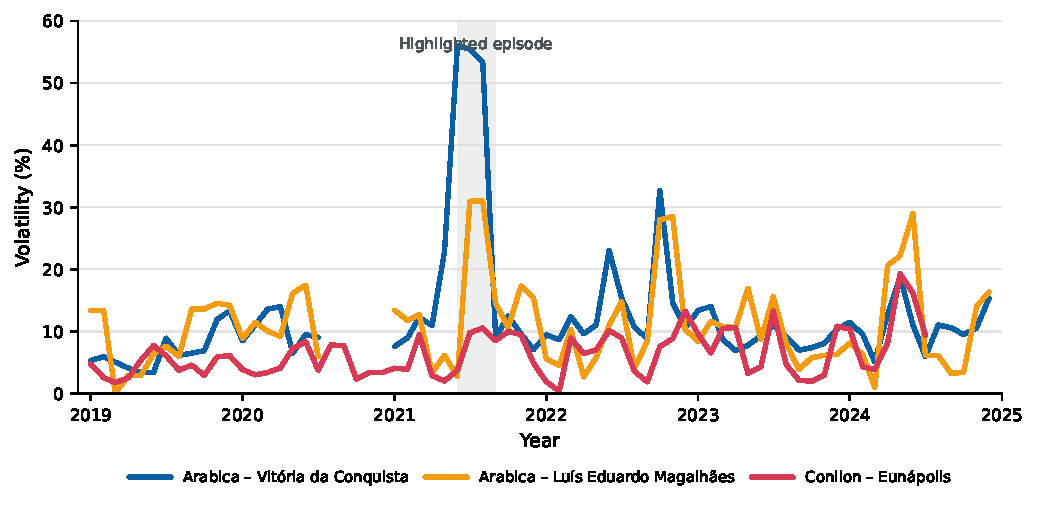
\includegraphics[width=\linewidth]{figs/coffee_bahia_volatility_intro.pdf}
\par\medskip
\noindent\textbf{Figure~\thefigure.} Observed upper-tail volatility of local coffee prices in Bahia, Brazil.
\end{minipage}
\end{center}
\label{fig:intro_volatility}

Given this gap, the \textbf{objective} of this study is to evaluate whether information from other agricultural commodities and from financial markets improves the out-of-sample forecasting of future volatility of local Arabica and Conilon coffee prices in Bahia, relative to models that use only the history of the local market itself. The analysis uses three local SEAGRI-BA series, corresponding to Arabica coffee in Vitória da Conquista, Arabica coffee in Luís Eduardo Magalhães and Conilon coffee in Eunápolis. To achieve this objective, the study addresses six research questions:

\begin{itemize}
\item[\textbf{RQ1.}] Do machine-learning models outperform traditional econometric models (GARCH and HAR-RV) in forecasting local coffee volatility?
\item[\textbf{RQ2.}] Does including information from other commodities (international coffee, the CEPEA indicator, soybean, cotton and cocoa) improve forecasts relative to own history?
\item[\textbf{RQ3.}] Do financial and macro-financial variables (exchange rate, interest rates, oil, financial volatility and stock indices) provide additional predictive gains?
\item[\textbf{RQ4.}] Do the relative performance of the models and the value of external information differ across low-, medium- and high-volatility regimes?
\item[\textbf{RQ5.}] Which variables and information blocks contribute most to the forecasts for each variety?
\item[\textbf{RQ6.}] Are the relevant drivers similar for Arabica and Conilon, or specific to each variety?
\end{itemize}

The questions are treated as an out-of-sample empirical evaluation, without presupposing the direction of the effects. Null or negative results are therefore informative for the selection of models and information sources. RQ1 compares model families; RQ2 and RQ3 isolate the value of each information block; RQ4 examines the stability of these results; and RQ5 and RQ6 identify the drivers associated with the forecasts.

The empirical design compares GARCH(1,1) and HAR-RV with Random Forest, XGBoost and LightGBM, estimated on four nested information sets. E1 uses only own history, E2 adds cross-commodity variables, E3 adds financial variables and E4 combines all blocks. This structure separates the effect of the algorithm from the effect of information. The evaluation uses strict expanding-window temporal validation, horizons of one, five and twenty observations, the QLIKE, MAE and RMSE losses, Diebold--Mariano tests with the Harvey--Leybourne--Newbold correction and multiple-comparison adjustments, analysis by regimes defined ex ante, and explainability through native importances and SHAP \citep{Wang2024SystemicRiskML,Diachkov2026FinancialStressML}.

The study makes three contributions to the commodity markets literature. First, it provides out-of-sample evidence on volatility forecasting in thinly traded local spot markets of an emerging economy, characterized by infrequent quotations and long gaps, a setting largely absent from a literature concentrated on futures contracts and international benchmarks. Second, it quantifies, through controlled ablation experiments, how much global commodity and financial information adds to local volatility forecasts, and shows that the value of financial information is regime dependent, which is consistent with an intermittent transmission of financial conditions to local physical markets. Third, it shows that simple econometric benchmarks remain hard to beat in this setting and that the importance assigned by machine-learning models to financial variables does not translate into predictive gains, a relevant caveat for risk managers and for the use of explainability tools in commodity finance.

The remainder of the article is organized as follows. Section~\ref{sec:materials_methods} describes the data, volatility measures, models and validation protocol. Section~\ref{sec:experiments} presents the experiments and their results, organized by research question. Section~\ref{sec:discussion} discusses the results in light of the literature and presents the limitations, and Section~\ref{sec:conclusion} concludes.

\section{Materials and Methods}
\label{sec:materials_methods}

This section describes a two-layer observational design. The first layer organizes local quotations, related commodities and financial indicators into a temporal panel. The second uses nested feature blocks to produce out-of-sample forecasts of the future volatility of local coffee prices with econometric and machine-learning models. The results are therefore interpreted as evidence of incremental information content and not as a causal decomposition of volatility.

\subsection{Study design}
\label{subsec:study_design}

The study is quantitative, longitudinal and based on time series of observed prices. The forecasting unit is an available quotation for a combination of variety and local market, identified by \(c\) and by the date \(t\). For each unit, the local price, past returns, historical volatility measures, the available external variables and the future volatility associated with horizon \(h\) are observed. Formally, the set of observations for series \(c\) is

\begin{equation}
\mathcal{D}_{c}=\left\{\left(t,P_{c,t},\mathbf{x}_{c,t},V_{c,t,h}\right)\;\middle|\;t\in\mathcal{T}_{c},\ h\in\{1,5,20\}\right\}.
\label{eq:data_unit}
\end{equation}

\refstepcounter{figure}
\begin{center}
\begin{minipage}{\textwidth}
\centering
\resizebox{\textwidth}{!}{%
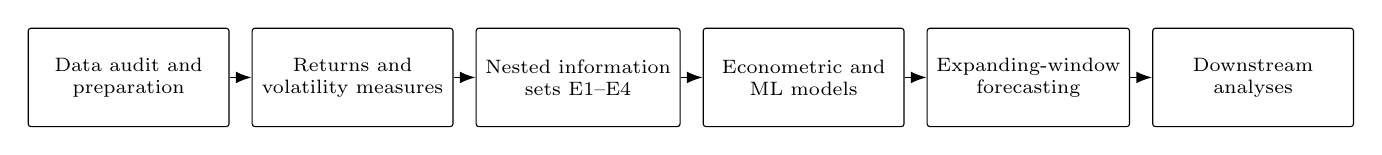
\begin{tikzpicture}[
  stage/.style={draw, rectangle, rounded corners=1pt, minimum width=2.55cm, minimum height=1.25cm, align=center, font=\scriptsize},
  flow/.style={-{Latex[length=2mm]}, line width=0.6pt}
]
\node[stage] (data) {Data audit and\\preparation};
\node[stage, right=0.28cm of data] (temporal) {Returns and\\volatility measures};
\node[stage, right=0.28cm of temporal] (sets) {Nested information\\sets E1--E4};
\node[stage, right=0.28cm of sets] (models) {Econometric and\\ML models};
\node[stage, right=0.28cm of models] (forecast) {Expanding-window\\forecasting};
\node[stage, right=0.28cm of forecast] (downstream) {Downstream\\analyses};
\draw[flow] (data) -- (temporal);
\draw[flow] (temporal) -- (sets);
\draw[flow] (sets) -- (models);
\draw[flow] (models) -- (forecast);
\draw[flow] (forecast) -- (downstream);
\end{tikzpicture}%
}
\noindent\textbf{Figure~\thefigure.} Study workflow: data preparation, volatility measures, nested information sets, model estimation, expanding-window forecasting and downstream analyses.
\end{minipage}
\end{center}
\label{fig:study_design}

The workflow in Figure~\ref{fig:study_design} organizes the analysis into six blocks. Data preparation structures local and external observations on a common temporal basis. The return and volatility measures transform prices into features comparable across units and define the forecasting target. The nested information sets E1--E4 separate own history, cross-commodity information and financial information. The econometric and machine-learning models are estimated on these sets, and expanding-window forecasting produces out-of-sample estimates for horizons of one, five and twenty observations. Finally, the downstream analyses evaluate predictive performance, statistical significance, heterogeneity across markets and regimes, and feature importance.

Because the local series contain days without updates and long intervals without observations, no artificial daily grid was created. Each horizon is counted in successive observations of the target series itself. This choice preserves the nature of the data and avoids turning periods without quotations into synthetic returns.

The dependent variables are Arabica coffee in the markets of Vitória da Conquista and Luís Eduardo Magalhães and Conilon coffee in the market of Eunápolis. To keep the comparison internally consistent, the Rio grade was selected for the two Arabica series and grade 7 for the Conilon series. After the cleaning described in Section~\ref{subsec:data_cleaning}, the panel contains 14,126 observations across the three series.

\begin{table*}[t]
\centering
\caption{Characteristics of the local series used as dependent variables}
\label{tab:target_series}
\scriptsize
\begin{tabular*}{\textwidth}{@{\extracolsep{\fill}}p{3.6cm}lrlrrr@{}}
\hline
Series & Grade & \(N\) & Period & \(s(r_t)\) & Median \(HVol_{5}\) & Median \(V_{20}\) \\
\hline
Arabica, Vitória da Conquista & Rio & 4,427 & 2001-12-03 to 2026-01-21 & 3.126 & 2.410 & 6.899 \\
Arabica, Luís Eduardo Magalhães & Rio & 4,195 & 2003-02-05 to 2026-01-21 & 3.066 & 0.000 & 6.899 \\
Conilon, Eunápolis & Grade 7 & 5,504 & 2001-12-14 to 2026-01-21 & 1.962 & 1.170 & 4.455 \\
\hline
\end{tabular*}
\end{table*}

Prices are expressed in Brazilian reais per 60-kg bag. Returns and the \(HVol_{5}\) and \(V_{20}\) measures are in percentage points. The twenty-period horizon corresponds to the next twenty available observations of the local series.

\subsection{Data sources and observed variables}
\label{subsec:data_sources}

Local prices were obtained from the Bahia State Department of Agriculture, Livestock, Irrigation, Fisheries and Aquaculture (SEAGRI-BA). The national reference price was obtained from the Center for Advanced Studies on Applied Economics (CEPEA), with Arabica and Robusta coffee series. International futures contracts were obtained from the continuous series provided by Yahoo Finance: ICE Coffee C \texttt{KC=F}, soybean \texttt{ZS=F}, cotton \texttt{CT=F} and cocoa \texttt{CC=F}. These series are treated as market references and not as automatic substitutes for an official series of individual contracts, since the continuity and roll-over convention belongs to the data source.

The financial and macro-financial variables were combined from public sources. The USD/BRL exchange rate and the SELIC rate annualized over 252 days were obtained from the Central Bank of Brazil. The VIX volatility index, the broad U.S. dollar index, the ten-year U.S. Treasury yield and the effective Fed Funds rate were obtained from Federal Reserve Economic Data. The Brent spot price was obtained from the U.S. Energy Information Administration. S\&P 500 and Ibovespa returns were computed from the corresponding historical series.

\subsubsection{Exploratory data analysis}
\label{subsec:eda}

Before integrating the sources and estimating the models, an exploratory data analysis was carried out along three dimensions. The first examined temporal coverage, the number of observations, median prices, the standard deviation of returns and the historical and future volatility measures. These results are presented in Table~\ref{tab:target_series}. The final panel contains 14,126 observations across the three local series. Median prices are 300.00, 310.00 and 247.00 reais per 60-kg bag for Vitória da Conquista, Luís Eduardo Magalhães and Eunápolis, respectively. The standard deviations of returns are 3.126, 3.066 and 1.962 percentage points, while the medians of \(V_{20}\) are 6.899, 6.899 and 4.455 percentage points. The coincidence of the \(V_{20}\) medians in the two Arabica series stems from the discreteness of quotations, which concentrates price changes on a few price steps, and not from identical series. On the 3,958 common dates, the prices of the two markets coincide on only 12.86\% of the dates and the correlation between returns is 0.137, although price levels are strongly correlated (0.991). Only 5.38\% of the common dates record a simultaneous price change in both markets.

The second dimension assessed the effective frequency of price updates. The shares of unchanged prices were 77.48\% in Vitória da Conquista, 87.56\% in Luís Eduardo Magalhães and 84.10\% in Eunápolis. A recorded date therefore does not necessarily represent a new transaction or a price change. This low update frequency carries over to the target: on the common evaluation support, future volatility is exactly zero in 76.9\% to 88.4\% of origins for \(h=1\), in 36.6\% to 53.0\% for \(h=5\) and in 5.8\% to 10.0\% for \(h=20\), depending on the series. This feature conditions the QLIKE evaluation and is addressed explicitly in the robustness analyses. The third dimension examined the evolution of volatility over time. Figure~\ref{fig:intro_volatility} highlights differences across markets and the June--August 2021 episode, when the monthly 90th percentile reached approximately 56\% in Vitória da Conquista, 31\% in Luís Eduardo Magalhães and 11\% in Eunápolis. The EDA was used to guide the definition of horizons, the interpretation of gaps and the choice of measures based on successive observations, without replacing temporal validation.

\subsubsection{Data audit and retention criteria}
\label{subsec:data_audit}

An automated audit was applied to 74 candidate series from SEAGRI-BA, CEPEA, the Central Bank of Brazil, Federal Reserve Economic Data, CBOE, the U.S. Energy Information Administration and Yahoo Finance. For each series, the audit recorded the source, temporal coverage, frequency, number of observations, share of missing values, duplicated dates, share of unchanged prices, longest gap between observations, average monthly observations, business-day coverage, unit changes, an initial anomaly rate and notes on data provenance. The generic screening classified 31 series as initially usable and 43 as unusable, mainly because of insufficient coverage, long gaps or unit inconsistency.

The usability indicator was treated as a diagnostic and not as an automatic exclusion of the predefined target series. The three local series were retained for their substantive relevance to the research question, and their limitations were incorporated into the empirical design. The longest gaps between observations were 374 days in Vitória da Conquista, 812 days in Luís Eduardo Magalhães and 217 days in Eunápolis. The initial anomaly rates were 0.23\%, 0.48\% and 0.25\%, respectively. This evidence justified not interpolating prices, counting horizons in successive observations and explicitly preserving missing values.

In the final panel, the CEPEA return has 58.18\% missing values because it starts in 2016, while the missing shares are 0.35\% for the USD/BRL return, 2.36\% for the VIX, 1.85\% for the Brent return, 2.79\% for the soybean return, 2.96\% for the cotton return and 2.97\% for the cocoa return. The available information and the missingness pattern were preserved so that the incremental contribution of each block could be evaluated under a common sample and imputation rule.

\subsection{Cleaning, quality control and temporal synchronization}
\label{subsec:data_cleaning}

Dates were converted to a standard temporal format, records were sorted and duplicated observations were grouped by date, keeping the last recorded quotation. No linear interpolation was applied to prices. The absence of a quotation was not interpreted as price stability and was not filled with a future observation.

We removed January 1 in every year, since quotations recorded on that date were incompatible with a regular trading day; the record of August 31, 2023, identified as a common failure of the SEAGRI-BA data feed; and an isolated point on July 28, 2010, in the Vitória da Conquista series, characterized by a jump and immediate reversal consistent with a decimal error. Other absolute returns above 40\% were kept and flagged by the indicator variable \texttt{is\_extreme\_return}. Keeping them avoids eliminating potentially informative movements in a study whose object is precisely extreme variation.

Each exogenous series was transformed on its own calendar before integration. For a date \(t\) of the target series, the exogenous observation used is

\begin{equation}
x_{j,t}^{*}=x_{j,\tau_j(t)},
\qquad
\tau_j(t)=\max\left\{s\leq t\;|\;t-s\leq 7\text{ days}\right\}.
\label{eq:asof}
\end{equation}

When no observation \(s\) satisfies the condition in Equation~\ref{eq:asof}, the value remains missing. Integration was performed by a backward temporal join with a seven-day tolerance. The procedure uses only information available up to the forecast date and avoids silent filling across prolonged gaps.

\subsection{Returns and volatility measures}
\label{subsec:returns_volatility}

Log returns define the statistical unit used to represent price dynamics and the forecasting target. They reduce the effect of nominal scale and make it possible to compare local markets with commodities and financial markets. From these returns, the historical measures summarize the recent intensity of price changes and feed the models with information available at origin \(t\), while the sum of future squared returns builds the target for each horizon. This separation between past information and future variation is essential to avoid temporal leakage and to interpret the gains from the additional information blocks.

For each series \(c\), let \(P_{c,t}>0\) be the price observed at the \(t\)-th quotation. The log return, in percentage points, is

\begin{equation}
r_{c,t}=100\ln\left(\frac{P_{c,t}}{P_{c,t-1}}\right).
\label{eq:log_return}
\end{equation}

The return at the first observation of each series is missing. For the exogenous price series, the same transformation was applied on their native calendars before the temporal join.

The historical variation measures used as features were computed exclusively from returns available up to \(t\). For a window \(k\), define

\begin{equation}
HVar_{c,t,k}=\sum_{j=0}^{k-1}r_{c,t-j}^{2}
\label{eq:hist_var}
\end{equation}

and

\begin{equation}
HVol_{c,t,k}=\sqrt{HVar_{c,t,k}}.
\label{eq:hist_vol}
\end{equation}

Windows \(k\in\{5,10,20\}\) were used. These measures are not computed with future returns and can therefore be used as information available at time \(t\).

The dependent variable represents the accumulated intensity of future price changes. For each horizon \(h\in\{1,5,20\}\), the forward quadratic variation is

\begin{equation}
Q_{c,t,h}=\sum_{i=1}^{h}r_{c,t+i}^{2}
\label{eq:forward_variance}
\end{equation}

and the aggregated future volatility is

\begin{equation}
V_{c,t,h}=\sqrt{Q_{c,t,h}}.
\label{eq:forward_vol}
\end{equation}

The index \(t+i\) denotes the next available observation of the target series, not necessarily the next calendar day. The supervised models are fitted directly to \(V_{c,t,h}\). The quantity \(Q_{c,t,h}=V_{c,t,h}^{2}\) is used to evaluate variance-specific losses, especially QLIKE. Because the data are predominantly daily and contain no intraday returns, the term aggregated future volatility is preferred to the interpretation as a classical intraday \textit{realized volatility} measure.

Together, these definitions produce the univariate reference of the study. The own-history set \(E1\) uses the available returns, their lags and \(HVol_{c,t,5}\), \(HVol_{c,t,10}\) and \(HVol_{c,t,20}\). This specification is the local-information baseline for measuring the incremental gain of cross-commodity and financial variables. In parallel, GARCH(1,1) and the adapted HAR-RV serve as econometric baselines, as they model volatility exclusively from local history under different assumptions about persistence and temporal aggregation. This subsection thus establishes the historical predictors, defines the future target and ensures comparability across horizons, while the following subsections assess whether additional algorithms and information sources improve on this reference.

\subsection{Feature construction and information sets}
\label{subsec:features}

The own-series features include \(r_{c,t}\), five return lags and the three historical measures \(HVol_{c,t,5}\), \(HVol_{c,t,10}\) and \(HVol_{c,t,20}\). The own-history block thus contains nine variables

\begin{equation}
\mathcal{I}^{L}_{c,t}
=
\left\{
r_{c,t},r_{c,t-1},\ldots,r_{c,t-5},
HVol_{c,t,5},HVol_{c,t,10},HVol_{c,t,20}
\right\}.
\label{eq:local_info}
\end{equation}

The cross-commodity block contains the return and five-period volatility of the other local variety, the returns and five-period volatilities of soybean, cotton and cocoa, and the returns of the international coffee contract and of the national CEPEA indicator

\begin{equation}
\mathcal{I}^{C}_{t}
=
\left\{
r^{other}_{t},HVol^{other}_{t,5},
r^{soy}_{t},HVol^{soy}_{t,5},
r^{cotton}_{t},HVol^{cotton}_{t,5},
r^{cocoa}_{t},HVol^{cocoa}_{t,5},
r^{ICEcoffee}_{t},r^{CEPEA}_{t}
\right\}.
\label{eq:cross_info}
\end{equation}

For the other-variety variable, the Conilon return corresponds to the Eunápolis series and the Arabica return corresponds to the available average of the two Arabica markets. The average is computed on the observed calendar before the join with the target series.

The financial and macro-financial block is

\begin{equation}
\begin{aligned}
\mathcal{I}^{F}_{t}
={}&\left\{
r^{USD/BRL}_{t},HVol^{USD/BRL}_{t,5},
SELIC_{t},VIX_{t},\Delta VIX_{t},
r^{Brent}_{t},r^{Dollar}_{t}, \right.\\
&\left. r^{S\&P500}_{t},r^{Ibovespa}_{t},
Treasury10Y_{t},FedFunds_{t}
\right\}.
\end{aligned}
\label{eq:financial_info}
\end{equation}

The four information specifications are

\begin{equation}
\mathcal{X}^{E1}_{t}=\mathcal{I}^{L}_{c,t}
\label{eq:e1}
\end{equation}

\begin{equation}
\mathcal{X}^{E2}_{t}=\mathcal{I}^{L}_{c,t}\cup\mathcal{I}^{C}_{t}
\label{eq:e2}
\end{equation}

\begin{equation}
\mathcal{X}^{E3}_{t}=\mathcal{I}^{L}_{c,t}\cup\mathcal{I}^{F}_{t}
\label{eq:e3}
\end{equation}

\begin{equation}
\mathcal{X}^{E4}_{t}=\mathcal{I}^{L}_{c,t}\cup\mathcal{I}^{C}_{t}\cup\mathcal{I}^{F}_{t}.
\label{eq:e4}
\end{equation}

E1 represents own history. E2 adds cross-commodity information. E3 adds financial information. E4 contains all blocks. This structure makes it possible to estimate the marginal gain of each source without confounding the comparison between algorithms with the comparison between information sets.

\subsection{Econometric benchmark models}
\label{subsec:econometric_models}

The econometric models provide the benchmarks against which the machine-learning models are evaluated. They offer a controlled representation of volatility predictability based exclusively on local history, without cross-commodity variables or financial indicators. GARCH(1,1) represents the persistence of conditional variance, EGARCH is used as a robustness analysis to allow asymmetric responses to positive and negative shocks, and the adapted HAR-RV represents the aggregation of variation at daily, weekly and monthly scales. All are estimated with the same target definition and under the same temporal validation protocol applied to the other models. This organization makes it possible to distinguish the gain associated with additional information from the gain associated with algorithmic flexibility. GARCH(1,1) and HAR-RV are the main benchmarks, while EGARCH extends the analysis to volatility asymmetry.

\subsubsection{GARCH}

The GARCH(1,1) model was estimated on the local return with zero conditional mean and normal innovations \citep{Bollerslev1986GARCH}

\begin{equation}
r_{c,t}=\sigma_{c,t}z_{c,t},
\qquad
z_{c,t}\sim\mathcal{N}(0,1).
\label{eq:garch_return}
\end{equation}

The conditional variance is

\begin{equation}
\sigma_{c,t}^{2}
=
\omega
+\alpha r_{c,t-1}^{2}
+\beta\sigma_{c,t-1}^{2}.
\label{eq:garch}
\end{equation}

The parameters are estimated on the training set of each annual window. The forecast of forward quadratic variation is obtained by summing the forecast conditional variances

\begin{equation}
\widehat{Q}^{GARCH}_{c,t,h}
=
\sum_{i=1}^{h}\widehat{\sigma}_{c,t+i\mid t}^{2},
\qquad
\widehat{V}^{GARCH}_{c,t,h}
=
\sqrt{\widehat{Q}^{GARCH}_{c,t,h}}.
\label{eq:garch_forecast}
\end{equation}

As a robustness check, an EGARCH(1,1,1) model~\citep{Nelson1991EGARCH}, which allows asymmetric responses to positive and negative shocks, was estimated under the same protocol, with Monte Carlo forecasts (1,000 paths, seed 42) for \(h>1\). Because of convergence failures in part of the windows, EGARCH is excluded from the primary common support.

\subsubsection{HAR-RV}

The HAR-RV baseline was implemented as a linear regression of aggregated future volatility on variation measures at daily, weekly and monthly scales \citep{Corsi2009HAR}

\begin{equation}
V_{c,t,h}
=
\beta_{0,h}
+\beta_{d,h}\lvert r_{c,t}\rvert
+\beta_{w,h}HVol_{c,t,5}
+\beta_{m,h}HVol_{c,t,20}
+\varepsilon_{c,t,h}.
\label{eq:har}
\end{equation}

The coefficients were obtained by ordinary least squares exclusively on the training data of each window. The specification adapts the HAR principle to the aggregated volatility measure available in the daily series. At least 250 training observations were required to estimate each baseline.

\subsection{Machine-learning models}
\label{subsec:ml_models}

The supervised models estimate future volatility from the information sets \(E1\)--\(E4\). The choice of tree-based methods stems from the tabular, heterogeneous and potentially nonlinear nature of the features, which combine returns, volatility measures, commodity prices and financial indicators. These models can also represent interactions without imposing a linear functional form and do not require feature scaling, which avoids unnecessary transformations in a dataset with different units and update frequencies.

Random Forest was included as a \textit{bagging} benchmark. Averaging many trees reduces the instability of an individual tree and provides a robust reference for nonlinear relationships and extreme observations. XGBoost was chosen as a gradient \textit{boosting} method, in which successive trees correct the errors of previous ones and can capture more concentrated interactions among predictors. LightGBM extends this comparison with a histogram-based \textit{boosting} implementation and efficient tree growth. Including two \textit{boosting} methods makes it possible to check whether the results depend on a specific implementation or remain consistent across algorithms with different construction mechanisms. Together, the three models contrast variance reduction, sequential residual learning and computational efficiency \citep{Breiman2001RandomForest,ChenGuestrin2016XGBoost,Ke2017LightGBM}.

An independent model was fitted for each information set, horizon and target series. This organization prevents the volatility distribution of one market from being used directly to fit another and makes it possible to assess whether the contribution of the features holds at horizons of one, five and twenty periods. Hyperparameters were fixed to control complexity, preserve reproducibility and prevent the limited number of observations per series from favouring excessively deep trees. For Random Forest, we used 100 estimators, a maximum depth of 6 and a minimum of 5 observations per leaf. The number of trees stabilizes the ensemble average, the depth allows moderate-order interactions and the minimum leaf size smooths predictions in regions with few observations.

For the \textit{boosting} models, we used 300 estimators and a learning rate of 0.05. The larger number of steps combined with small updates builds the forecast gradually and reduces reliance on overly aggressive corrections. For XGBoost, the maximum depth was 4, while for LightGBM it was 5. This difference preserves moderate complexity in both cases, given their different growth strategies. For LightGBM, a minimum of 10 observations per leaf was additionally required, which limits the formation of very specific regions. The random state was fixed at 42 in all models. No scaling was applied, since tree decisions depend on split points and not on the numerical distance between variables.

For each information set \(S\), horizon \(h\) and algorithm \(m\), a function was estimated

\begin{equation}
\widehat{V}^{m,S}_{c,t,h}
=
\widehat{f}^{m,S}_{c,h}\left(\mathcal{X}^{S}_{t}\right).
\label{eq:ml_general}
\end{equation}

Three tree-based models were used \citep{Breiman2001RandomForest,ChenGuestrin2016XGBoost,Ke2017LightGBM}. Random Forest combines \(B\) regression trees

\begin{equation}
\widehat{f}_{RF}(\mathbf{x})
=
\frac{1}{B}\sum_{b=1}^{B}T_b(\mathbf{x}),
\label{eq:rf}
\end{equation}

while the boosting models form an additive function

\begin{equation}
\widehat{f}_{Boost}(\mathbf{x})
=
\sum_{b=1}^{B}\eta g_b(\mathbf{x}),
\label{eq:boost}
\end{equation}

where \(g_b\) is a sequentially added tree and \(\eta\) is the learning rate.

Missing feature values were imputed with the training-set median. For each variable \(j\), the transformation was

\begin{equation}
x^{imp}_{j,t}
=
\begin{cases}
x_{j,t}, & \text{if }x_{j,t}\text{ is observed} \\
\operatorname{median}\left(x_{j,t}\mid t\in\mathcal{T}_{train}\right), & \text{if }x_{j,t}\text{ is missing}.
\end{cases}
\label{eq:imputation}
\end{equation}

The medians were recomputed in each window and were never estimated with test observations. Forecasts were bounded below at \(10^{-6}\) to guarantee a positive quantity in the variance transformation.

\subsection{Temporal validation and prevention of data leakage}
\label{subsec:temporal_validation}

Forecasts were evaluated by temporal validation with an expanding training window and annual re-estimation. For a test year \(y\), the cutoff is

\begin{equation}
C_y=\text{January 1 of year }y.
\label{eq:cutoff}
\end{equation}

The training set for horizon \(h\) is

\begin{equation}
\mathcal{T}_{y,h}
=
\left\{
t
\;\middle|\;
\text{date}_{c,t}<C_y,\;
\text{date}_{c,t+h}<C_y,\;
V_{c,t,h}\text{ observed}
\right\}.
\label{eq:train_set}
\end{equation}

The test set is

\begin{equation}
\mathcal{E}_{y,h}
=
\left\{
t
\;\middle|\;
\text{year}(\text{date}_{c,t})=y,\;
V_{c,t,h}\text{ observed}
\right\}.
\label{eq:test_set}
\end{equation}

This rule removes from training the labels whose future period reaches the test year. The first forecast of each series occurs after at least three full years of history, and each fit requires at least 250 valid observations. For GARCH and EGARCH, the parameters are estimated once per annual window and held fixed during the test year. The variance recursion is updated at each origin with returns observed up to \(t\), without changing the estimated parameters. For HAR-RV and the machine-learning models, fitting is likewise performed only with training observations.

The same temporal principle was applied to data preparation. The temporal join, imputation and fitting of each algorithm are carried out within each window. The final comparison uses dates common to all primary configurations, so that a performance difference is not produced by different test samples. The common validation support comprises 12,541 forecasts for \(h=1\), 12,529 for \(h=5\) and 12,484 for \(h=20\).

\subsection{Forecast evaluation metrics}
\label{subsec:metrics}

Forecast quality is compared across models, information sets, target series and horizons. More than one measure is needed because future volatility is evaluated on two related but non-equivalent scales. The variance scale is appropriate for assessing the quality of quadratic-risk forecasts, while the volatility scale preserves the unit in which accumulated returns are interpreted. Table~\ref{tab:forecast_metrics} summarizes the role of each metric and its relation to the empirical questions of the study.

\begin{table*}[t]
\centering
\caption{Forecast evaluation metrics and analytical indicators used in the study}
\label{tab:forecast_metrics}
\scriptsize
\setlength{\tabcolsep}{2pt}
\begin{tabular*}{\textwidth}{@{\extracolsep{\fill}}p{1.8cm}p{2.4cm}p{4.7cm}p{6.1cm}@{}}
\hline
Metric & Scale and direction & What it emphasizes & Question addressed in the study \\
\hline
QLIKE & Variance \(Q=V^{2}\), lower is better & Evaluates variance forecasts through the relative error between \(Q\) and \(\widehat{Q}\). It is the main measure for comparing quadratic-risk forecasts. & Which model best represents the intensity of future risk when the target is treated as a variance measure, and which information reduces this loss the most? \\
\hline
MAE & Volatility, lower is better & Measures the mean absolute error on the same scale as \(V\). It offers a direct interpretation of the typical error and is less sensitive to large isolated deviations. & Which model produces forecasts closest to observed volatility on average, and which results remain interpretable in the unit of the phenomenon? \\
\hline
RMSE & Volatility, lower is better & Squares errors before averaging and gives more weight to large failures. It is especially informative for stress episodes and severe underestimation. & Which model best reduces extreme errors and maintains performance in the riskiest periods? \\
\hline
Incremental gains \(G_C\), \(G_F\) and \(G_{CF}\) & Relative loss reduction, higher is better & Compares the baseline loss with the loss after adding cross-commodity, financial or combined information. & Does external information add predictability beyond own history? \\
\hline
\end{tabular*}
\end{table*}

The volatility-evaluation literature shows that there is no universal ranking of models independent of the loss function. \citet{HansenLunde2006ConsistentRanking} show that rankings can be inconsistent when an inadequate proxy is used to represent conditional variance and recommend out-of-sample evaluations with more informative volatility measures. \citet{Patton2011VolatilityProxy} shows that comparisons can be distorted when the volatility proxy is imperfect and identifies a class of losses robust to this noise, in which QLIKE plays a central role. Reviews of agricultural commodity forecasting also indicate that results depend on the horizon, frequency, model specification and validation protocol \citep{Guindani2024AgriculturalForecasting}. These results justify the joint use of QLIKE, MAE and RMSE in this study.

For each forecast, let \(V_{c,t,h}\) be the observed volatility, \(\widehat{V}_{c,t,h}\) the forecast, \(Q_{c,t,h}=V_{c,t,h}^{2}\) the observed variance and \(\widehat{Q}_{c,t,h}=\widehat{V}_{c,t,h}^{2}\) the forecast variance. The QLIKE loss was computed as

\begin{equation}
\operatorname{QLIKE}_{c,t,h}
=
\frac{Q_{c,t,h}}{\widehat{Q}_{c,t,h}}
-\ln\left(\frac{Q_{c,t,h}}{\widehat{Q}_{c,t,h}}\right)-1.
\label{eq:qlike}
\end{equation}

Because there are observations with zero returns and, consequently, \(Q_{c,t,h}=0\), both observed and forecast variances were bounded below by \(\epsilon=10^{-4}\) before applying Equation~\ref{eq:qlike}. Because the share of zero targets is high, especially at \(h=1\), the floor can dominate the value of the loss in these observations. The QLIKE ranking of the models was therefore re-examined in two robustness exercises: (i) varying the floor over \(\epsilon\in\{10^{-4},10^{-2},10^{-1},1\}\) and (ii) restricting the evaluation to origins with \(Q_{c,t,h}>0\), where the floor does not affect the observed variance. Incremental gains were also recomputed on pooled losses, that is, as the ratio of aggregated mean losses, which prevents extreme ratios from a single series from dominating the average. QLIKE is the main measure for evaluating variance forecasts, while MAE and RMSE are computed on the volatility scale

\begin{equation}
\operatorname{MAE}
=
\frac{1}{n}\sum_{t=1}^{n}
\left\lvert V_{c,t,h}-\widehat{V}_{c,t,h}\right\rvert
\label{eq:mae}
\end{equation}

and

\begin{equation}
\operatorname{RMSE}
=
\sqrt{
\frac{1}{n}\sum_{t=1}^{n}
\left(V_{c,t,h}-\widehat{V}_{c,t,h}\right)^{2}
}.
\label{eq:rmse}
\end{equation}

To measure incremental predictability, let \(R_S\) be the mean out-of-sample loss for set \(S\). The relative gain from adding cross-commodity information, financial information and both blocks is

\begin{equation}
G_C=\frac{R_{E1}-R_{E2}}{R_{E1}},
\qquad
G_F=\frac{R_{E1}-R_{E3}}{R_{E1}},
\qquad
G_{CF}=\frac{R_{E1}-R_{E4}}{R_{E1}}.
\label{eq:incremental_gain}
\end{equation}

The conditional gains are also computed

\begin{equation}
G_{C\mid F}=\frac{R_{E3}-R_{E4}}{R_{E3}},
\qquad
G_{F\mid C}=\frac{R_{E2}-R_{E4}}{R_{E2}}.
\label{eq:conditional_gain}
\end{equation}

Positive values indicate a reduction in mean loss and negative values indicate a deterioration of the forecast after the information block is added. The interpretation is predictive, not causal.

\subsection{Predictive comparison tests}
\label{subsec:dm_test}

Predictive comparison checks whether the observed differences in forecast metrics are large enough to be distinguished from sampling variation. Comparing two mean losses may suggest that one configuration is better, but the difference may not replicate in other test samples. The Diebold--Mariano test evaluates the null hypothesis of equal mean predictive accuracy between two configurations, while the Harvey--Leybourne--Newbold correction adjusts inference in finite samples and in situations where forecast errors are serially dependent \citep{DieboldMariano1995,HarveyLeybourneNewbold1997}.

This correction is particularly important in this study because the five- and twenty-period targets are built from overlapping future returns. Forecasts issued on nearby dates may share part of the same future interval, so their loss differentials are not independent. Estimating the variance with autocovariances up to \(h-1\) and Bartlett weights reduces the risk of declaring statistical superiority on the basis of underestimated standard errors. The tests are applied separately for each series, horizon, pair of configurations and loss function, always on the dates common to the compared forecasts.

To compare two configurations \(A\) and \(B\), the volatility errors are defined as

\begin{equation}
e^{A}_{t}=V_{c,t,h}-\widehat{V}^{A}_{c,t,h},
\qquad
e^{B}_{t}=V_{c,t,h}-\widehat{V}^{B}_{c,t,h}.
\label{eq:forecast_errors}
\end{equation}

For the squared-error, absolute-error and QLIKE losses, the loss differential is, respectively,

\begin{equation}
d_t^{SE}=(e^{A}_{t})^{2}-(e^{B}_{t})^{2},
\label{eq:dm_se}
\end{equation}

\begin{equation}
d_t^{AE}=\lvert e^{A}_{t}\rvert-\lvert e^{B}_{t}\rvert
\label{eq:dm_ae}
\end{equation}

and

\begin{equation}
d_t^{QLIKE}
=
\ell^{QLIKE}_{A,t}-\ell^{QLIKE}_{B,t}.
\label{eq:dm_qlike}
\end{equation}

The null hypothesis is equal mean predictive accuracy \citep{DieboldMariano1995,HarveyLeybourneNewbold1997}. To accommodate the serial dependence associated with overlapping horizons, the variance of the mean of \(d_t\) was estimated with autocovariances up to \(h-1\) and Bartlett weights

\begin{equation}
\widehat{\operatorname{Var}}(\bar d)
=
\frac{1}{n}
\left[
\widehat{\gamma}_{0}
+2\sum_{k=1}^{h-1}
\left(1-\frac{k}{h}\right)\widehat{\gamma}_{k}
\right],
\label{eq:dm_variance}
\end{equation}

where

\begin{equation}
\widehat{\gamma}_{k}
=
\frac{1}{n}
\sum_{t=k+1}^{n}
(d_t-\bar d)(d_{t-k}-\bar d).
\label{eq:dm_covariance}
\end{equation}

The Diebold--Mariano statistic with the Harvey--Leybourne--Newbold correction is

\begin{equation}
DM_{HLN}
=
\frac{\bar d}{\sqrt{\widehat{\operatorname{Var}}(\bar d)}}
\sqrt{
\frac{n+1-2h+h(h-1)/n}{n}
}.
\label{eq:dm_hln}
\end{equation}

The \(p\)-values are two-sided and computed from a Student \(t\) distribution with \(n-1\) degrees of freedom. The tests are carried out on the dates common to the two compared configurations, for each series, horizon, model and loss function.

Because the design produces 891 comparisons, individual significance at 5\% overstates the number of genuine differences. The \(p\)-values were therefore also adjusted with the Holm procedure, which controls the family-wise error rate, and with the Benjamini--Hochberg procedure, which controls the false discovery rate, both applied to the full set of 891 comparisons \citep{Holm1979,BenjaminiHochberg1995}. The QLIKE tests were repeated on the origins with \(Q_{c,t,h}>0\).

Rejecting the null hypothesis indicates a difference in mean predictive accuracy but does not establish causality; the \(p\)-values are therefore interpreted jointly with the magnitude of the gains, the loss function and the horizon.

\subsection{Heterogeneity, explainability and reproducibility}
\label{subsec:additional_analyses}

This subsection describes three complementary analyses: performance across volatility regimes and stress periods, the relative contribution of variables and information blocks, and the computational setup required for reproduction.

\subsubsection{Volatility regimes and stress periods}
\label{subsec:regimes}

Performance heterogeneity was examined across three volatility regimes. The main classification is defined \textit{ex ante}, based on the historical volatility available at the forecast origin. For each series \(c\) and test year \(y\), let \(\tilde q_{33,c,y}\) and \(\tilde q_{66,c,y}\) be the 33.33th and 66.67th percentiles of \(HVol_{c,s,20}\) computed only with dates \(s<C_y\). The regime of origin \(t\) is

\begin{equation}
Z_{c,t}
=
\begin{cases}
\mathrm{Low}, & HVol_{c,t,20}\leq \tilde q_{33,c,y} \\
\mathrm{Medium}, & \tilde q_{33,c,y}<HVol_{c,t,20}\leq \tilde q_{66,c,y} \\
\mathrm{High}, & HVol_{c,t,20}>\tilde q_{66,c,y}.
\end{cases}
\label{eq:regimes}
\end{equation}

This definition uses only information available at the origin and corresponds to what a user could observe when issuing the forecast. A classification based on observed future volatility, that is, on terciles of \(V_{c,t,h}\), would condition on the outcome itself and would mechanically favour, in the high tercile, models that forecast high variances. This \textit{ex post} classification is kept only as a descriptive decomposition. The regimes are not used as features and play no role in training.

To test formally whether the value of external information depends on the regime, the loss differential \(d_t=\ell_{E1,t}-\ell_{Ek,t}\), positive when block \(Ek\) improves the forecast, was regressed on indicators for the medium and high regimes, with the low regime as reference. The coefficient on the high regime measures the difference between the gain in the high regime and in the low regime. Standard errors were estimated with the Newey--West method with \(\max(5,h)\) lags to accommodate the serial dependence induced by overlapping horizons and by infrequent price updates \citep{NeweyWest1987}. Four historical intervals were also analysed: pre-2020, the COVID-19 shock in 2020, the frost and supply crisis of 2021--2022 and the post-2023 normalization.

\subsubsection{Feature importance and explainability}
\label{subsec:explainability}

The explainability analysis was applied to experiments E2 and E4 for the three tree-based models and horizons \(h\in\{1,5,20\}\). The native importances of the tree-based models were recorded for each feature and normalized within each fit. For LightGBM, the SHAP tree explainer was used \citep{LundbergLee2017SHAP}. For an observation \(\mathbf{x}\), the decomposition is

\begin{equation}
f(\mathbf{x})
=
\phi_{0}
+\sum_{j=1}^{p}\phi_{j}(\mathbf{x}),
\label{eq:shap_decomposition}
\end{equation}

where \(\phi_j(\mathbf{x})\) is the contribution of feature \(j\) to the forecast for that observation. The global importance of the feature was computed as the mean absolute value

\begin{equation}
S_j
=
\frac{1}{n}\sum_{i=1}^{n}
\left\lvert\phi_j(\mathbf{x}_i)\right\rvert
\label{eq:shap_global}
\end{equation}

and normalized by

\begin{equation}
\widetilde{S}_j
=
\frac{S_j}{\sum_{\ell=1}^{p}S_{\ell}}.
\label{eq:shap_normalized}
\end{equation}

The explainability models are fitted on the valid observations available for each series and horizon, with median imputation from the descriptive sample itself. This analysis does not replace out-of-sample evaluation. Its purpose is to identify which variables drive the forecasts and how importance is distributed across own history, cross-commodity information and financial variables.

\subsubsection{Implementation and reproducibility}
\label{subsec:reproducibility}

The pipeline was run in Python 3.12.10 with pandas 3.0.5, NumPy 2.5.2, arch 8.0.0, scikit-learn 1.9.0, LightGBM 4.7.0, XGBoost 3.4.1 and shap 0.52.0. Panel construction, baselines, machine-learning experiments, temporal validation, statistical tests, regime analysis, explainability and robustness checks were run in separate scripts, and all results were saved to CSV files for auditing. A run manifest records package versions, file hashes and the main parameters. The individual forecasts record the origin date, the end date of the horizon, the last training date, the cutoff and the validity of the forecast. The robustness analyses are run on the saved out-of-sample forecasts, without re-estimating the models.

\section{Experiments and Results}
\label{sec:experiments}

This section describes the empirical execution of the pipeline and presents, immediately after each element of the design, the corresponding results and discussion. The design was organized to separate three sources of predictive difference. The first is algorithmic flexibility, comparing econometric benchmarks and machine-learning models. The second is information content, comparing the series' own history with cross-commodity and financial blocks. The third is forecast stability, examined by horizon, market, volatility regime and stress period. The experimental unit is the combination of target series, horizon, origin date, information set and model.

\subsection{Experimental scope and comparison matrix}
\label{subsec:experimental_scope}

The experiments used the master dataset with 14,126 observations from three local series: Arabica coffee, Rio grade, in Vitória da Conquista and Luís Eduardo Magalhães, and Conilon coffee, grade 7, in Eunápolis. For each series, forecasts were generated for \(h=1\), \(h=5\) and \(h=20\) future observations. Each forecast was issued after the observed close at \(t\), using only features available up to that origin.

The primary comparison consisted of GARCH(1,1), HAR-RV, Random Forest, LightGBM and XGBoost. EGARCH(1,1,1) was run as a robustness check but was not included in the primary common support because of convergence failures in some windows. The machine-learning models were combined with four nested information sets. E1 contains nine own-history features, E2 contains these features plus ten cross-commodity features, E3 contains own history plus eleven financial features and E4 combines the thirty available features of the three blocks. This organization produces twelve machine-learning configurations and makes it possible to attribute performance differences to the algorithm or to the added information block. In the tables, the label E0 denotes the econometric baselines GARCH(1,1) and HAR-RV, which use only the return history of the series itself.

\begin{table*}[t]
\centering
\caption{Experimental matrix used in the validated comparison}
\label{tab:experimental_matrix}
\scriptsize
\setlength{\tabcolsep}{2pt}
\begin{tabular*}{\textwidth}{@{\extracolsep{\fill}}p{2.0cm}p{3.5cm}p{5.9cm}p{3.6cm}@{}}
\hline
Block & Configurations & Implementation & Purpose \\
\hline
Series and horizons & Three local series and \(h=1,5,20\) & Time unit defined by the next available observation of the target series & Measure heterogeneity across markets and horizons \\
\hline
Baselines & GARCH(1,1) and HAR-RV & Annual estimation with expanding window and at least 250 training observations & Set econometric benchmarks for local predictability \\
\hline
Econometric robustness & EGARCH(1,1,1) & Simulation with seed 42 and exclusion of non-convergent forecasts & Check whether asymmetry changes the comparison without replacing the primary support \\
\hline
Machine learning & Random Forest, LightGBM and XGBoost & Fixed hyperparameters, training-median imputation and deterministic execution with seed 42 & Evaluate nonlinear relationships and feature interactions \\
\hline
Information & E1, E2, E3 and E4 & Nine, nineteen, twenty and thirty features, respectively & Quantify incremental gains from own history, commodities and finance \\
\hline
Evaluation & QLIKE, MAE and RMSE & Dates common to all primary configurations and losses computed by series and horizon & Compare quadratic risk, typical error and large-amplitude failures \\
\hline
Diagnostics & DM-HLN, regimes and importance & Tests on three losses with Holm and Benjamini--Hochberg corrections, \textit{ex ante} regimes with HAC tests, historical periods, native importances and SHAP & Examine significance, stability and information content \\
\hline
Robustness & QLIKE floor and zero targets & \(\epsilon\in\{10^{-4},10^{-2},10^{-1},1\}\), evaluation restricted to \(Q>0\) and gains on pooled losses & Check whether the ranking depends on the treatment of zero targets \\
\hline
\end{tabular*}
\end{table*}

\subsection{Model estimation and computational setup}
\label{subsec:experiment_implementation}

GARCH(1,1) was fitted to the returns of the target series in each annual window, and its forecasts were updated recursively with returns observed up to the origin. HAR-RV was estimated by least squares using the daily absolute return and historical measures over five- and twenty-observation windows. EGARCH followed the same temporal separation and used 1,000 simulations for horizons longer than one period. Its parameters remained fixed during each test year.

The tabular models were fitted separately for each combination of series, horizon, information set and annual window. Random Forest used 100 trees, a maximum depth of 6 and a minimum of five observations per leaf. LightGBM used 300 trees, a maximum depth of 5, a learning rate of 0.05 and a minimum of ten observations per leaf. XGBoost used 300 trees, a maximum depth of 4 and a learning rate of 0.05. All algorithms used \texttt{random\_state=42} and a single processing unit. No hyperparameter optimization was performed at this stage. Fixing the values keeps model complexity constant and focuses the comparison on the effect of the algorithm and of the information sets.

Before fitting, missing features were imputed with the median computed exclusively on the training set. The same transformation was applied to the test set without recomputing the median. Volatility forecasts were bounded below at \(10^{-6}\), while the floor \(\epsilon=10^{-4}\) was applied to variances in the QLIKE loss. These controls prevent negative forecasts and numerical problems associated with windows of zero returns.

\subsection{Temporal validation, leakage control and evaluation coverage}
\label{subsec:experimental_validation}

The protocol used an expanding training window and an annual test cycle. The first window was formed after three years of available observations, and each fit required at least 250 valid observations. In each year, all features, imputations and supervised parameters were defined within the training window. The test set remained separate until the forecast was generated.

Because the horizon-\(h\) target uses returns after the origin, training was purged whenever the last observation needed to build the label reached the test year. The audit recorded 186 combinations of series, horizon and test year and removed 1,578 labels potentially overlapping the evaluation period. The individual forecasts kept the origin, the end of the horizon, the last training date, the cutoff and the validity indicator. This information made it possible to verify that no supervised label used observations after the cutoff.

A total of 37,554 forecasts were attempted for each configuration, summing over the three series and three horizons. The primary configurations produced 100\% valid forecasts. EGARCH had 95.26\% aggregate validity because of convergence limitations and was kept out of the primary comparison for this reason. For the main comparison, only the dates on which all primary configurations had a valid forecast were kept. The common support comprised 12,541 dates for \(h=1\), 12,529 for \(h=5\) and 12,484 for \(h=20\), ensuring that error differences were not produced by different samples.

\subsection{Pooled performance: baselines vs.\ machine learning}
\label{subsec:results_coverage}

The evaluation was carried out on both the volatility and the variance scales. QLIKE was computed with the numerical floor defined in the methodology and served as the main measure of quadratic risk. MAE measured the absolute distance between observed and forecast volatility. RMSE gave additional weight to large-amplitude errors. Pooled aggregation gave equal weight to each individual forecast over the 12,541, 12,529 and 12,484 dates of the common support described in Section~\ref{subsec:experimental_validation}.

Table~\ref{tab:pooled_results} summarizes the winning configurations for each horizon and loss function. GARCH(1,1) had the lowest QLIKE at all three horizons, with values of 9.374, 6.362 and 2.606. HAR-RV had the lowest MAE and RMSE at all horizons, with MAE of 1.074, 2.783 and 5.254 and RMSE of 2.442, 4.992 and 8.697. This result shows that the ranking of models depends on the evaluation scale. GARCH was favoured when the comparison prioritized variance, while HAR-RV was favoured when the interest lay in the distance between forecast and observed volatility.

\begin{table}[t]
\centering
\caption{Pooled winning configurations by horizon and loss}
\label{tab:pooled_results}
\scriptsize
\setlength{\tabcolsep}{2pt}
\begin{tabular}{@{}p{0.65cm}p{1.05cm}p{2.55cm}r@{}}
\hline
\(h\) & Loss & Winning configuration & Value \\
\hline
1 & QLIKE & E0--GARCH(1,1) & 9.374 \\
1 & MAE & E0--HAR-RV & 1.074 \\
1 & RMSE & E0--HAR-RV & 2.442 \\
5 & QLIKE & E0--GARCH(1,1) & 6.362 \\
5 & MAE & E0--HAR-RV & 2.783 \\
5 & RMSE & E0--HAR-RV & 4.992 \\
20 & QLIKE & E0--GARCH(1,1) & 2.606 \\
20 & MAE & E0--HAR-RV & 5.254 \\
20 & RMSE & E0--HAR-RV & 8.697 \\
\hline
\end{tabular}
\end{table}

Among the machine-learning models, Random Forest had the most consistent aggregate performance. For QLIKE, its best configurations were E2 at \(h=1\), with 20.437, E2 at \(h=5\), with 7.754, and E1 at \(h=20\), with 3.373. For MAE, E1 was the best configuration at \(h=1\) and \(h=5\), with 1.109 and 2.934, while E2 was the best at \(h=20\), with 5.440. For RMSE, E2 was the best configuration at \(h=1\) and \(h=20\), with 2.478 and 9.236, and E1 was the best at \(h=5\), with 5.194. Even as the best machine-learning model, Random Forest remained above HAR-RV in pooled MAE and RMSE. The gap narrowed at the twenty-observation horizon but did not disappear.

The boosting models showed greater instability under QLIKE. LightGBM had high pooled losses at all three horizons, while XGBoost alternated relative gains in some configurations with high losses in others. This difference between families should not be interpreted as a universal superiority of Random Forest, since the results depend on the loss function and the market. It indicates that nonparametric flexibility alone does not replace the need for an econometric benchmark suited to the scale of risk.

Figure~\ref{fig:pooled_comparison} displays this pooled comparison, showing QLIKE (on a logarithmic scale), MAE and RMSE by horizon for the two baselines and the best configuration of each machine-learning family. The figure illustrates the ranking reversal between QLIKE and the volatility-scale metrics and the greater dispersion of LightGBM and XGBoost under QLIKE.

\refstepcounter{figure}
\begin{center}
\begin{minipage}{\textwidth}
\centering
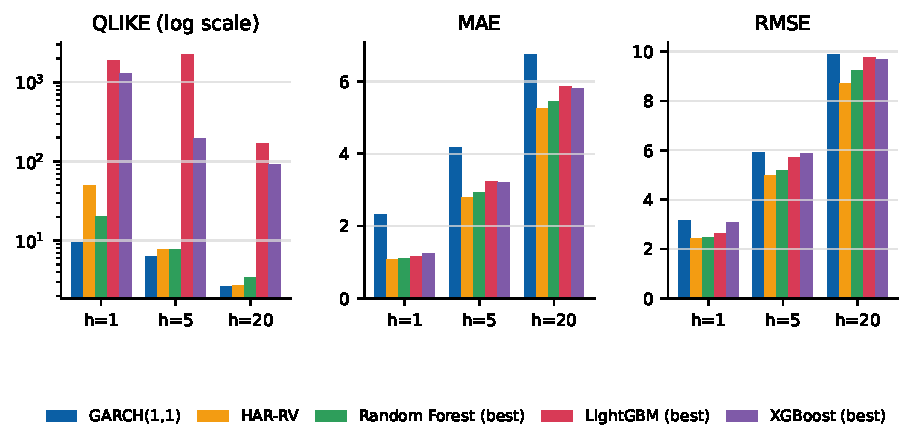
\includegraphics[width=\textwidth]{figs/fig_pooled_comparison.pdf}
\par\medskip
\noindent\textbf{Figure~\thefigure.} Pooled QLIKE, MAE and RMSE by horizon for GARCH(1,1), HAR-RV and the best configuration of each machine-learning family.
\end{minipage}
\end{center}
\label{fig:pooled_comparison}

\subsection{Robustness of QLIKE to zero targets}
\label{subsec:results_qlike_robustness}

Because future volatility is zero in a large share of origins, especially at \(h=1\), the absolute values of pooled QLIKE are high and depend on the floor \(\epsilon\). To check whether the ranking of models is an artefact of this floor, Table~\ref{tab:qlike_robust} reports pooled QLIKE with \(\epsilon=1\) and restricted to origins with \(Q_{c,t,h}>0\).

\begin{table}[t]
\centering
\caption{QLIKE robustness: pooled QLIKE of GARCH(1,1), HAR-RV and the best machine-learning configuration under alternative variance floors and on non-zero targets}
\label{tab:qlike_robust}
\scriptsize
\setlength{\tabcolsep}{2pt}
\begin{tabular}{@{}p{1.55cm}p{0.4cm}rrrrl@{}}
\hline
Scenario & \(h\) & \(n\) & GARCH & HAR-RV & Best ML & Configuration \\
\hline
\(\epsilon=10^{-4}\) & 1 & 12,541 & 9.374 & 49.990 & 20.437 & E2--RF \\
 & 5 & 12,529 & 6.362 & 7.636 & 7.754 & E2--RF \\
 & 20 & 12,484 & 2.606 & 2.688 & 3.373 & E1--RF \\
\hline
\(\epsilon=1\) & 1 & 12,541 & 1.956 & 5.382 & 3.950 & E4--XGB \\
 & 5 & 12,529 & 2.332 & 3.658 & 3.781 & E2--RF \\
 & 20 & 12,484 & 1.888 & 1.970 & 2.656 & E1--RF \\
\hline
\(Q>0\) & 1 & 2,131 & 7.810 & 258.759 & 84.806 & E2--RF \\
 & 5 & 7,033 & 2.518 & 5.629 & 5.846 & E2--RF \\
 & 20 & 11,525 & 1.765 & 1.879 & 2.638 & E1--RF \\
\hline
\end{tabular}
\end{table}

GARCH(1,1) had the lowest pooled QLIKE in all scenarios and horizons, including the intermediate values \(\epsilon=10^{-2}\) and \(\epsilon=10^{-1}\), not reported in the table. The magnitude of the losses decreases as the floor increases or as zero targets are excluded, but the ranking of GARCH, HAR-RV and the best machine-learning model remains unchanged. On the origins with price changes, GARCH also had the lowest MAE and RMSE at \(h=1\), with 2.305 and 5.002, while HAR-RV kept the lowest volatility-scale losses at \(h=5\) and \(h=20\). This indicates that part of HAR-RV's MAE advantage at the short horizon stems from low forecasts at origins without price changes. The DM-HLN QLIKE tests restricted to origins with \(Q_{c,t,h}>0\) confirm the pattern: no machine-learning configuration was significantly better than GARCH or HAR-RV, and 66 of the 108 comparisons with GARCH were significantly in favour of GARCH. GARCH's QLIKE advantage is therefore not an artefact of the treatment of zero targets.

\subsection{Results by market and horizon}
\label{subsec:results_heterogeneity}

The decomposition by series confirms the heterogeneity observed in the EDA and addresses whether predictability holds across locations. GARCH had the lowest QLIKE in eight of the nine combinations of series and horizon. The exception was Luís Eduardo Magalhães at the twenty-observation horizon, where HAR-RV had a QLIKE of 2.488, lower than GARCH. HAR-RV had the lowest RMSE in all nine combinations and the lowest MAE in eight. The MAE exception also occurred in Luís Eduardo Magalhães at \(h=20\), where E2 with Random Forest had an MAE of 6.665, against 6.682 for HAR-RV.

The advantage of the econometric benchmarks under QLIKE was clearest at the short and intermediate horizons. At the long horizon, forecasts became closer in some markets and cross-commodity information became competitive for Random Forest. In Luís Eduardo Magalhães, E2 with Random Forest had an MAE of 6.665 and an RMSE of 9.203 at \(h=20\). In Vitória da Conquista and Eunápolis, however, HAR-RV kept the lowest volatility-scale losses. The differences across markets reinforce that the usefulness of external features is not homogeneous and must be evaluated by series and horizon.

\subsection{Incremental value of the information blocks}
\label{subsec:results_incremental}

The incremental comparisons were computed with E1 as the reference for each series, horizon and algorithm, so that the gain of E2, E3 or E4 represents the relative loss reduction associated with the new information block. Cross-commodity information was the most consistent external block for Random Forest. As shown in Table~\ref{tab:rf_incremental}, E2 reduced Random Forest's QLIKE in all three series at \(h=1\), in two series at \(h=5\) and in only one series at \(h=20\). On the volatility scale, E2 improved MAE in one series at the short horizon, in one at the intermediate horizon and in two at the long horizon. RMSE was reduced in two series at the short horizon, in one at the intermediate horizon and in all three series at the long horizon.

\begin{table}[t]
\centering
\caption{Incremental gains from cross-commodity information for Random Forest}
\label{tab:rf_incremental}
\scriptsize
\setlength{\tabcolsep}{2pt}
\begin{tabular}{@{}p{2.15cm}p{0.55cm}rrr@{}}
\hline
Series & \(h\) & QLIKE (\%) & MAE (\%) & RMSE (\%) \\
\hline
Arabica LEM & 1 & 3.94 & -1.02 & -0.20 \\
Arabica LEM & 5 & 8.75 & 3.22 & 2.39 \\
Arabica LEM & 20 & 2.96 & 4.28 & 4.57 \\
Arabica VDC & 1 & 5.57 & 1.70 & 1.08 \\
Arabica VDC & 5 & 1.66 & -2.88 & -4.10 \\
Arabica VDC & 20 & -8.41 & 0.90 & 3.20 \\
Conilon Eunápolis & 1 & 6.40 & -3.34 & 0.18 \\
Conilon Eunápolis & 5 & -1.86 & -2.48 & -1.30 \\
Conilon Eunápolis & 20 & -3.02 & -1.51 & 1.68 \\
\hline
\end{tabular}
\end{table}

The mean gains of E2 for Random Forest were 5.30\% in QLIKE at the short horizon, 2.85\% at the intermediate horizon and -2.82\% at the long horizon. For MAE, the mean gains were -0.89\%, -0.71\% and 1.22\%. For RMSE, they were 0.35\%, -1.00\% and 3.15\%. These values show that adding related commodities can improve forecasts in certain markets but does not produce a uniform gain across metrics.

The financial block did not deliver a systematic improvement over own history. For Random Forest, the mean gains of E3 were negative in QLIKE at all three horizons and also in MAE and RMSE. The full set E4 reproduced this pattern, with negative mean gains for Random Forest in all three metrics.

The results for LightGBM and XGBoost show that instability under QLIKE is more intense in the boosting models. The simple average of relative gains by series, used above for Random Forest, becomes uninformative for these models, because a single series with an explosive loss dominates the average. Table~\ref{tab:ml_incremental_pooled} therefore reports gains computed on pooled losses, that is, \(1-\bar R_{Ek}/\bar R_{E1}\), where \(\bar R\) is the aggregated mean loss over the three series.

\begin{table*}[t]
\centering
\caption{Incremental gains (\%) over E1 computed on pooled losses, by model, information block and horizon (\(\epsilon=10^{-4}\))}
\label{tab:ml_incremental_pooled}
\scriptsize
\setlength{\tabcolsep}{3pt}
\begin{tabular*}{\textwidth}{@{\extracolsep{\fill}}llrrrrrrrrr@{}}
\hline
 & & \multicolumn{3}{c}{QLIKE} & \multicolumn{3}{c}{MAE} & \multicolumn{3}{c}{RMSE} \\
Model & Block & \(h=1\) & \(h=5\) & \(h=20\) & \(h=1\) & \(h=5\) & \(h=20\) & \(h=1\) & \(h=5\) & \(h=20\) \\
\hline
Random Forest & E2 & 5.59 & 2.42 & -4.20 & -0.63 & -0.59 & 1.43 & 0.47 & -1.33 & 3.29 \\
Random Forest & E3 & -3.42 & -9.77 & -8.20 & -7.46 & -8.78 & -15.08 & -4.04 & -10.04 & -19.66 \\
Random Forest & E4 & 0.01 & -6.60 & -5.64 & -5.78 & -5.32 & -16.73 & -2.51 & -8.28 & -19.50 \\
LightGBM & E2 & -39.13 & 29.01 & -660.67 & -3.01 & -3.16 & 3.50 & -1.74 & -4.43 & 5.37 \\
LightGBM & E3 & -179.37 & -138.98 & 60.30 & -4.77 & -17.54 & -7.16 & -3.33 & -17.82 & -12.28 \\
LightGBM & E4 & -151.52 & -6.77 & -39.47 & -4.68 & -12.12 & -6.01 & -2.70 & -14.24 & -9.82 \\
XGBoost & E2 & 72.21 & 91.53 & -649.28 & 5.76 & 0.65 & 1.40 & 20.43 & 1.84 & 6.24 \\
XGBoost & E3 & 73.16 & 44.42 & -47.13 & -6.18 & -13.14 & -10.84 & 21.73 & -9.36 & -9.75 \\
XGBoost & E4 & 64.21 & 28.61 & -861.13 & -2.66 & -9.07 & -12.40 & 24.20 & -5.63 & -10.71 \\
\hline
\end{tabular*}
\end{table*}

Three patterns emerge. First, for Random Forest, the cross-commodity block produces small gains of varying sign, positive in QLIKE at the short and intermediate horizons and in MAE and RMSE at the long horizon. Second, the financial and full blocks worsen MAE and RMSE in all models at the twenty-observation horizon, with losses between 6\% and 20\%. Third, the QLIKE gains of the boosting models alternate between large positive values and losses of several hundred percent. XGBoost's positive gains at \(h=1\) and \(h=5\) mainly reflect the weakness of that model's E1 configuration rather than good absolute performance, since no XGBoost configuration comes close to the losses of GARCH or HAR-RV. Restricting the evaluation to origins with \(Q_{c,t,h}>0\), the patterns hold: Random Forest's QLIKE gain with E2 is 7.90\%, 5.46\% and -5.86\% at the three horizons, and blocks E3 and E4 remain negative at \(h=5\) and \(h=20\). Hence, only the cross-commodity block in Random Forest yields gains of stable, albeit small, magnitude, and financial information does not translate into predictive gains.

Figure~\ref{fig:incremental_gains} summarizes Random Forest's gains by information block and horizon, computed on pooled losses. Random Forest is the only model whose QLIKE gains remain on an interpretable scale across the three blocks. The cross-commodity block (E2) is the only one that preserves a positive mean QLIKE gain at the short and intermediate horizons, while the financial (E3) and full (E4) blocks produce mean losses in practically all combinations of metric and horizon, confirming that additional information does not necessarily imply predictive gains.

\refstepcounter{figure}
\begin{center}
\begin{minipage}{\textwidth}
\centering
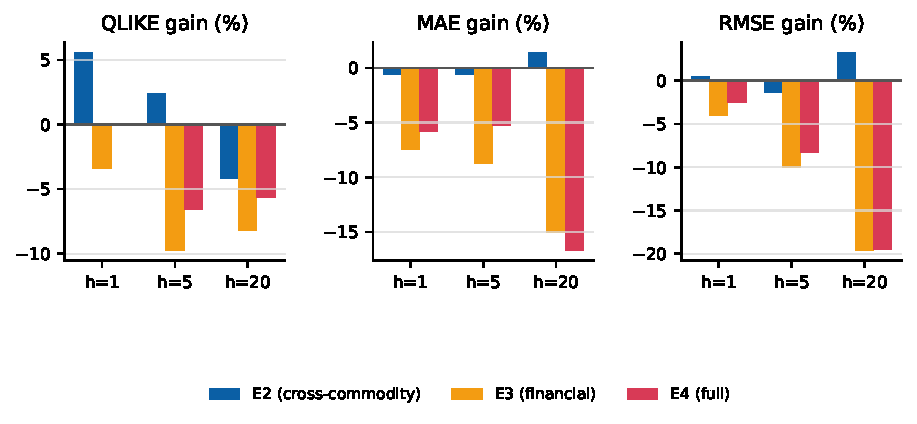
\includegraphics[width=\textwidth]{figs/fig_incremental_gains.pdf}
\par\medskip
\noindent\textbf{Figure~\thefigure.} Incremental gains of Random Forest over the E1 own-history baseline, computed on pooled losses, by information block (E2, E3, E4) and horizon.
\end{minipage}
\end{center}
\label{fig:incremental_gains}

\subsection{Predictive superiority comparisons (DM-HLN tests)}
\label{subsec:results_statistical_tests}

Performance differences were tested with the Diebold--Mariano test with the Harvey--Leybourne--Newbold correction. Squared losses, absolute losses and QLIKE were evaluated. The first set of comparisons examined E1 against E2, E3 and E4 within each machine-learning family. The second compared each machine-learning configuration with HAR-RV and GARCH(1,1). The direction of the differential was kept alongside the \(p\)-value to distinguish improvement, statistical tie and deterioration.

The DM-HLN tests recorded in \texttt{statistical\_tests\_results.csv} produced 891 comparisons on the same temporal support used in the evaluation, formed by series, horizon, model pair and loss function. Within the machine-learning families, the differences between E1 and the extended blocks were significant in 54 of 81 MAE comparisons, 53 of 81 squared-error comparisons and 10 of 81 QLIKE comparisons. However, only 13 MAE comparisons and eight squared-error comparisons were significantly in favour of the extended set. No significant QLIKE difference favoured E2, E3 or E4. The statistical evidence therefore supports localized incremental gains, but not a general superiority of external information.

The comparisons with the baselines reinforce the dependence on the loss function. In QLIKE, no machine-learning configuration was significantly better than GARCH or HAR-RV. In MAE, 88 of the 108 comparisons between machine learning and GARCH were significantly in favour of the machine-learning model, while no comparison with HAR-RV was significantly in favour of machine learning. In squared error, 40 comparisons were significantly in favour of machine learning against GARCH and none against HAR-RV. Machine-learning models can therefore outperform GARCH in part of the volatility-scale comparisons, but do not outperform HAR-RV in a statistically significant way on that scale.

Table~\ref{tab:dm_tests} consolidates these 891 DM-HLN comparisons into counts by comparison type and loss function, with and without multiple-comparison corrections.

\begin{table}[t]
\centering
\caption{DM-HLN test outcomes by comparison type and loss function: raw 5\% significance and after Benjamini--Hochberg (BH) and Holm corrections over the 891 tests}
\label{tab:dm_tests}
\scriptsize
\setlength{\tabcolsep}{2pt}
\begin{tabular}{@{}p{2.2cm}p{0.8cm}rrrrrrr@{}}
\hline
 & & & \multicolumn{2}{c}{5\%} & \multicolumn{2}{c}{BH} & \multicolumn{2}{c}{Holm} \\
Comparison & Loss & N & Sig. & Fav. & Sig. & Fav. & Sig. & Fav. \\
\hline
E1 vs.\ E2/E3/E4 & MAE & 81 & 54 & 13 & 49 & 11 & 30 & 2 \\
E1 vs.\ E2/E3/E4 & RMSE & 81 & 53 & 8 & 46 & 6 & 22 & 3 \\
E1 vs.\ E2/E3/E4 & QLIKE & 81 & 10 & 0 & 9 & 0 & 0 & 0 \\
ML vs.\ GARCH(1,1) & MAE & 108 & 94 & 88 & 93 & 87 & 77 & 73 \\
ML vs.\ GARCH(1,1) & RMSE & 108 & 68 & 40 & 60 & 40 & 39 & 32 \\
ML vs.\ GARCH(1,1) & QLIKE & 108 & 65 & 0 & 59 & 0 & 16 & 0 \\
ML vs.\ HAR-RV & MAE & 108 & 94 & 0 & 87 & 0 & 69 & 0 \\
ML vs.\ HAR-RV & RMSE & 108 & 99 & 0 & 96 & 0 & 48 & 0 \\
ML vs.\ HAR-RV & QLIKE & 108 & 43 & 0 & 37 & 0 & 11 & 0 \\
\hline
\end{tabular}
\end{table}

In the first three rows, ``Fav.'' counts significant comparisons in favour of the extended information set (E2, E3 or E4) over E1. In the remaining rows, it counts significant comparisons in favour of the machine-learning model over the corresponding econometric baseline. Significant differences that are not favourable correspond to deteriorations.

The multiple-comparison correction substantially reduces the evidence in favour of external information. Under the Holm criterion, which controls the probability of at least one false positive among the 891 comparisons, only two MAE comparisons and three squared-error comparisons remain significantly in favour of the extended sets, against 28 and 19 significantly unfavourable comparisons. Under the less conservative Benjamini--Hochberg criterion, 11 and 6 favourable comparisons remain. In contrast, the superiority of HAR-RV over the machine-learning models and GARCH's QLIKE advantage survive both corrections. For Random Forest with E2, the comparisons significantly in favour at 5\% were 3 of 9 in MAE, 1 of 9 in squared error and none in QLIKE.

\subsection{Volatility regimes and stress periods}
\label{subsec:results_regimes}

Heterogeneity was examined with regimes defined \textit{ex ante} by terciles of historical volatility \(HVol_{c,t,20}\), with thresholds estimated only with data prior to each test year (Equation~\ref{eq:regimes}). The low regime contains 5,730 origins per horizon, and the medium and high regimes contain about 3,500 and 3,300 origins, respectively. The asymmetry stems from the decline in historical volatility in the most recent years relative to thresholds estimated on earlier history.

The ranking of the models remained stable across regimes. GARCH had the lowest pooled QLIKE in all three regimes, with 6.336, 5.997 and 5.871 in the low, medium and high regimes, and also on origins with price changes, with 2.426, 2.691 and 2.910. The best machine-learning model, always a Random Forest configuration, recorded QLIKE between 9.799 and 10.722. In MAE, HAR-RV was the best benchmark in all three regimes, with 2.823, 2.908 and 3.535, practically tied with Random Forest with E2 in the low regime, at 2.826. The advantage of the econometric benchmarks therefore does not depend on the regime.

The value of external information, by contrast, depends strongly on the regime. Figure~\ref{fig:regime_analysis} shows the MAE gain of each block over E1, computed on pooled losses within each regime. In the low regime, the financial and full blocks worsen MAE by 20\% to 27\% in all models. In the medium regime, the losses shrink to 2\% to 8\%. In the high regime, the gains become positive, between 1.8\% and 7.6\% for E3 and between 0.7\% and 7.4\% for E4. The cross-commodity block, in contrast, shows small and roughly stable gains across regimes, between -1.7\% and 2.5\%.

\refstepcounter{figure}
\begin{center}
\begin{minipage}{\textwidth}
\centering
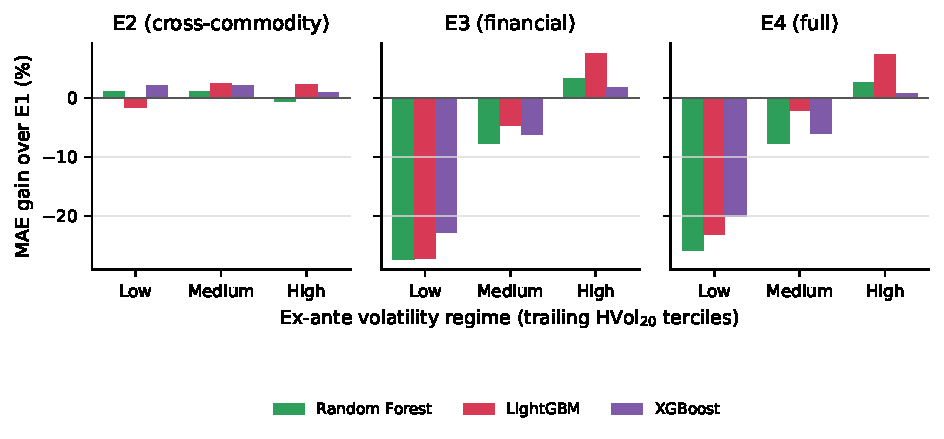
\includegraphics[width=\textwidth]{figs/fig_regime_analysis.pdf}
\par\medskip
\noindent\textbf{Figure~\thefigure.} MAE gain over the E1 own-history baseline by ex-ante volatility regime (terciles of trailing \(HVol_{20}\), thresholds estimated before each test year), by information block and model. Gains are computed on pooled losses.
\end{minipage}
\end{center}
\label{fig:regime_analysis}

The HAC tests confirm this pattern. For the financial and full blocks, the difference between the gain in the high regime and in the low regime was positive and significant at 5\% in 6 to 7 of the 9 combinations of series and horizon in MAE for each model, and in 3 to 5 of the 9 in squared error, with at most one significant difference in the opposite direction. For the cross-commodity block, significant differences were rare and of opposite signs, between one and three per model and loss. In QLIKE restricted to origins with price changes, almost no difference between regimes was significant.

This result indicates that financial variables are not useless under all conditions. They worsen the forecast in calm periods, when local volatility is low and movements in financial markets do not pass through to local quotations, and they start to add information in periods of high volatility. Because calm regimes predominate in the sample, the average effect is negative. The \textit{ex post} decomposition, based on terciles of future volatility, suggested the opposite pattern, with cross-commodity gains concentrated in the high regime and negative financial gains in all regimes. This divergence illustrates the bias of conditioning the evaluation on the outcome and justifies using the \textit{ex ante} classification as the main analysis.

The decomposition by historical periods produced a pattern consistent with the stability of the benchmarks. GARCH had the lowest mean QLIKE before 2020, during the COVID-19 shock, during the 2021--2022 frost and supply crisis and in the post-2023 period, with means of 6.73, 4.54, 4.96 and 4.42. The period analysis does not establish causality for the events, but identifies how forecasting difficulty changes over time.

\subsection{Feature importance and interpretation of the results}
\label{subsec:results_explainability}

Explainability was computed for E2 and E4 for the three tree-based models and the three horizons. The native importances of Random Forest, LightGBM and XGBoost were normalized and aggregated into own history, cross-commodity and financial variables. SHAP was computed with \texttt{TreeExplainer} for LightGBM and exported together with the feature importances, producing 441 feature records and 30 group aggregates.

The native importances show a shift in information composition as the horizon increases. In E2, the mean aggregate importance of own history was 0.055, 0.053 and 0.054 for \(h=1\), \(h=5\) and \(h=20\), while cross-commodity importance was 0.050, 0.052 and 0.051. In the E4 set, the financial block had the highest mean importance at \(h=20\), with 0.051, above own history, with 0.028, and the cross-commodity block, with 0.019. This result suggests that financial variables may gain relevance at longer horizons, even without producing a systematic improvement in aggregate loss.

Figure~\ref{fig:feature_importance} compares the composition of mean importance by feature group in E2 and E4 at the three horizons. In E2, own history and cross-commodity remain close and stable across horizons. In E4, the importance of the financial block increases monotonically with the horizon and overtakes the other blocks at \(h=20\), while the importance of own history declines.

\refstepcounter{figure}
\begin{center}
\begin{minipage}{\textwidth}
\centering
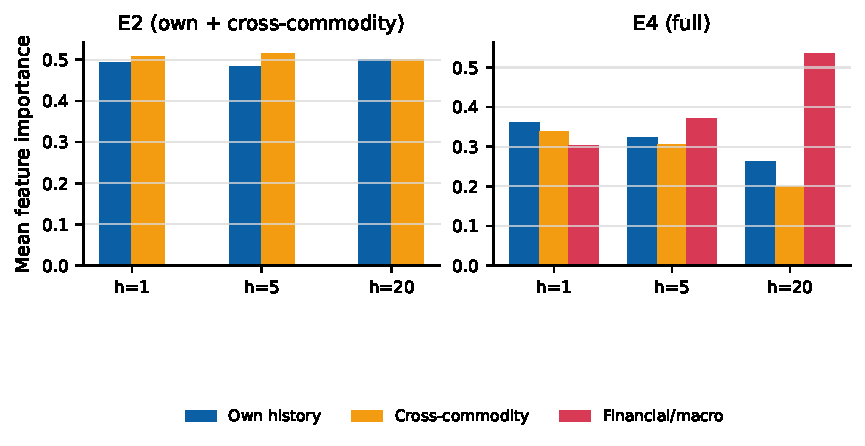
\includegraphics[width=\textwidth]{figs/fig_feature_importance.pdf}
\par\medskip
\noindent\textbf{Figure~\thefigure.} Mean feature-group importance by horizon for the E2 and E4 information sets, averaged across varieties and tree-based models.
\end{minipage}
\end{center}
\label{fig:feature_importance}

Among individual features, \texttt{return\_lag4} and \texttt{cepea\_return} were among the most important at \(h=1\) in the E2 set. At \(h=5\) and \(h=20\), \texttt{hist\_vol\_20} remained among the main features in E2. In E4, \texttt{selic} was the feature with the highest mean importance at the five- and twenty-observation horizons. These importances are diagnostics of relative contribution within the models and do not represent elasticities or causal effects.

The LightGBM SHAP values confirm this pattern and make it sharper. With equal weight for the three series, the share of the financial block in E4 was 0.386, 0.499 and 0.672 at \(h=1\), \(h=5\) and \(h=20\), while own history fell from 0.279 to 0.190 and the cross-commodity block from 0.335 to 0.138. In E2, own history and cross-commodity remained balanced, with cross-commodity shares of 0.559, 0.504 and 0.497. The features with the highest mean SHAP in E4 were \texttt{selic}, \texttt{fed\_funds} and \texttt{us\_treasury\_10y} at \(h=5\) and \(h=20\), with the SELIC reaching 0.251 at \(h=20\). In E2, \texttt{cepea\_return} led at \(h=1\) and \texttt{hist\_vol\_20} at \(h=5\) and \(h=20\).

This result must be interpreted with caution. The most important financial variables are interest-rate levels, which evolve slowly and follow long-term trends. In tree-based models fitted on an expanding window, these levels can act as markers of the sample period, which helps explain the combination of high importance and no out-of-sample gain for E3 and E4 (Table~\ref{tab:ml_incremental_pooled}). Similarly, the importance of \texttt{cepea\_return} may partly reflect its missingness pattern before 2016. Moreover, the native and SHAP importances are computed on the full descriptive sample and measure contribution to the fit, not to out-of-sample accuracy.

Figure~\ref{fig:feature_importance} pools Arabica and Conilon, which may hide variety-specific differences. Figure~\ref{fig:variety_importance} disaggregates the same composition by variety for the E4 set. For Arabica, financial importance already exceeds own history and cross-commodity at \(h=5\) and becomes dominant at \(h=20\). For Conilon, the financial block is the least important at \(h=1\) and \(h=5\) and becomes dominant only at \(h=20\), while cross-commodity importance declines monotonically across the three horizons. Because importances are normalized to sum to one in each fit, the comparison between varieties relies only on the relative composition of the blocks, not on absolute magnitude. These results indicate that the relevant drivers are not interchangeable between the two varieties.

\refstepcounter{figure}
\begin{center}
\begin{minipage}{\textwidth}
\centering
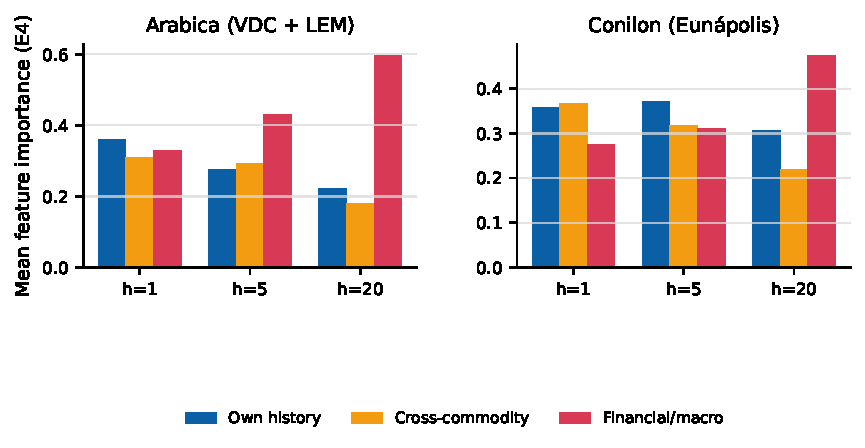
\includegraphics[width=\textwidth]{figs/fig_variety_importance.pdf}
\par\medskip
\noindent\textbf{Figure~\thefigure.} Mean feature-group importance by horizon for the E4 information set, disaggregated by coffee variety (Arabica vs.\ Conilon).
\end{minipage}
\end{center}
\label{fig:variety_importance}

\section{Discussion}
\label{sec:discussion}

The results presented in Section~\ref{sec:experiments} show a consistent picture: the econometric benchmarks were not beaten, cross-commodity information added only marginal gains and financial information worsened the forecasts on average, with a value that depends on the volatility regime. This section discusses why this pattern emerges and what it means. Section~\ref{subsec:disc_benchmarks} examines the factors that make the econometric benchmarks hard to beat in this setting. Section~\ref{subsec:disc_conditional} interprets the conditional value of external information in light of the literature on connectedness between markets. Section~\ref{subsec:disc_practical} translates the results into guidance for coffee market participants, and Section~\ref{subsec:disc_limitations} presents the limitations of the study.

\subsection{Why econometric benchmarks remain hard to beat}
\label{subsec:disc_benchmarks}

The main conclusion of the study is that simple econometric models, estimated only with local history, were not outperformed by more flexible machine-learning models or by broader information sets. This result contrasts with studies reporting gains from hybrid and machine-learning models in forecasting agricultural volatility and prices \citep{Manogna2025HybridVolatility,Zhang2025ClimateRealizedVolatility,Jin2024CoffeePriceML}, but it is consistent with reviews showing that the gains of these models depend on the market, the data frequency, the horizon and the validation protocol \citep{Guindani2024AgriculturalForecasting}. Three features of the present design help explain the difference.

The first is the nature of the series. SEAGRI-BA local quotations remain unchanged on 77\% to 88\% of dates, and future volatility is zero in most short-term origins. Under these conditions, the relevant dynamics resemble a sequence of sparse jumps rather than a continuous process with rich nonlinear interactions. The advantage of flexible models depends on the existence of complex and stable patterns not captured by own history, which is unlikely in series with this information density.

The second is the alignment between the estimation loss and the evaluation loss. GARCH is estimated by Gaussian quasi-maximum likelihood, whose implicit loss coincides with QLIKE, whereas HAR-RV is estimated by least squares on volatility and directly minimizes a quadratic loss on the evaluated scale. The tree-based models, in turn, were trained with squared error on volatility and do not incorporate the asymmetry of QLIKE, which heavily penalizes variance underestimation. This alignment, discussed by \citet{Patton2011VolatilityProxy} and \citet{HansenLunde2006ConsistentRanking}, explains why each benchmark wins on the scale for which it was estimated and why the ranking depends on the loss function.

The third is the temporal stability of the relationships. The most important external variables in the models, interest-rate levels, evolve slowly and follow long-term trends. In trees fitted on an expanding window, these variables allow the sample to be partitioned by period, which improves the in-sample fit but does not generalize to test years with interest-rate levels outside the historical range. The combination of high SHAP importance and out-of-sample losses is consistent with this mechanism.

\subsection{Conditional value of external information}
\label{subsec:disc_conditional}

The regime results offer a more precise interpretation of the role of financial information. The connectedness literature shows that volatility transmission between commodities and financial markets intensifies during crises and stress periods \citep{Singh2026OilSoftCommoditySpillovers,Zhou2026CommodityConnectedness}, and the financialization literature shows that co-movement with financial markets increased mainly for commodities included in investment indices~\citep{TangXiong2012,ChengXiong2014}. Local spot markets for a specific coffee grade are far removed from this channel. The results of this study are consistent with this evidence at the local scale: financial information harms the forecast when local volatility is low and adds information when it is high. In calm periods, movements in exchange rates, interest rates or stock indices are interpreted by the models as risk signals that do not materialize in local quotations, producing overly volatile forecasts. In turbulent periods, integration between markets increases and these signals come to contain relevant information.

Cross-commodity information behaved differently, with small and stable gains across regimes. The most important variables in this block, the CEPEA indicator and the international coffee contract, are directly linked to local price formation. Even so, two markets of the same variety, subject to the same market references, show a correlation of only 0.137 between their returns and simultaneous price changes on only 5.38\% of common dates. This pattern indicates that local quotations incorporate market references with delay and irregularly, which limits the contemporaneous predictive content of external variables. This finding is consistent with evidence that local policies and conditions have limited capacity to contain swings driven by external forces, but also that the transmission of these forces to regional markets is not immediate \citep{Fahmi2023LocalCoffeePolicy,AliagaMiranda2026CoffeeShocks}, as emphasized by the spatial price analysis literature~\citep{FacklerGoodwin2001}.

Finally, the stability of GARCH across stress periods contrasts with evidence that traditional GARCH specifications may have limitations in periods of instability \citep{Brun2026GARCHCoffeeRisk}. In the present setting, GARCH's QLIKE advantage held before 2020, during the COVID-19 shock, during the 2021--2022 frost and supply crisis and in the subsequent period. This difference may reflect the fact that the present study evaluates aggregated variance forecasts at short horizons, not extreme-risk measures.

\subsection{Practical implications}
\label{subsec:disc_practical}

For producers, cooperatives and marketing agents, the results suggest model selection guided by the purpose of the forecast. When the goal is to size risk in variance terms, as in computing margins or value-at-risk measures, GARCH(1,1) offers the most reliable benchmark. When the goal is to anticipate the typical magnitude of price changes, HAR-RV has the lowest errors. Adding external variables to machine-learning models should not be treated as an automatic improvement. Cross-commodity information can be kept for its low cost and marginal gain, while financial information is justified only in periods of high volatility, which suggests combination or selection strategies conditioned on the regime. For policymakers and development lenders, the results caution against importing volatility signals from futures or financial markets into local risk-monitoring systems without regime-specific validation.

\subsection{Limitations}
\label{subsec:disc_limitations}

The results should be interpreted in light of some limitations. First, local quotations are infrequent and contain long gaps, so observed volatility is dominated by sparse jumps and zero targets. Although the robustness analyses show that the ranking of models does not depend on the treatment of these targets, a two-stage model separating the probability of a price change from the magnitude of the change could better capture this structure. Second, the machine-learning models were estimated with fixed hyperparameters and a squared loss on volatility. This choice preserves comparability across information sets but does not exhaust the potential of these models, which could be tuned by nested temporal validation or trained with losses aligned with QLIKE. Third, GARCH was estimated with normal innovations, and heavy-tailed distributions may be more appropriate for series with jumps. Fourth, the interest-rate variables entered in levels, and the native and SHAP importances were computed in sample; using changes and out-of-sample permutation importances would better separate predictive value from fit. Fifth, the temporal join uses the last observation available up to the date of the local quotation, and it is not possible to verify whether the close of external markets on the same date precedes the collection of the SEAGRI-BA quotation. Sixth, the study covers three series from a single state, and the international contracts were obtained as continuous Yahoo Finance series, whose roll-over convention belongs to the source. Finally, the evaluation is statistical and does not include measures of economic value, such as the performance of hedging strategies or value-at-risk backtesting.

\subsection{Synthesis of the discussion}

Taken together, the discussion indicates that the weaker performance of the machine-learning models does not stem from an isolated specification failure, but from the combination of local series with low information density, estimation losses misaligned with evaluation losses and external variables whose relationship with local volatility is not stable over time. This reading also explains why external information is not uniformly useless. Its value appears when integration between markets intensifies, as in high-volatility periods, and disappears when local quotations evolve disconnected from financial markets. The contribution of the study is therefore not only to show that more flexible models and broader information sets do not guarantee better forecasts, but to identify under which conditions and through which mechanisms this information can be useful. The limitations identified define the agenda for testing whether this pattern holds with models trained for the relevant loss, with transformed financial variables and with evaluations of the economic value of the forecasts, issues taken up in the conclusion.

\section{Conclusion}
\label{sec:conclusion}

This study evaluated whether information from other agricultural commodities and from financial markets improves the out-of-sample forecasting of future volatility of local Arabica and Conilon coffee prices in Bahia. Using three SEAGRI-BA series, four nested information sets, econometric and machine-learning models and strict temporal validation, the study showed that the answer is, in general, negative. Table~\ref{tab:rq_summary} summarizes the answer to each research question and the evidence supporting it.

\begin{table*}[t]
\centering
\caption{Summary of the answers to the research questions}
\label{tab:rq_summary}
\scriptsize
\setlength{\tabcolsep}{3pt}
\begin{tabular*}{\textwidth}{@{\extracolsep{\fill}}p{3.4cm}p{2.1cm}p{7.6cm}p{2.2cm}@{}}
\hline
Research question & Answer & Main evidence & Reference \\
\hline
RQ1. Does ML outperform the econometric models? & No & GARCH has the lowest QLIKE and HAR-RV the lowest MAE and RMSE at all horizons; no ML configuration is significantly better than HAR-RV under any loss, nor than GARCH in QLIKE; the result is robust to the QLIKE floor and to excluding zero targets & Tables~\ref{tab:pooled_results}, \ref{tab:qlike_robust}, \ref{tab:dm_tests} \\
\hline
RQ2. Do other commodities improve forecasts? & Marginally & Small gains of varying sign, restricted to Random Forest (QLIKE +5.6\% and +2.4\% at \(h=1\) and \(h=5\)); after the Holm correction, only 2 MAE and 3 squared-error comparisons favour the extended blocks & Tables~\ref{tab:rf_incremental}, \ref{tab:ml_incremental_pooled}, \ref{tab:dm_tests} \\
\hline
RQ3. Do financial variables add predictive gains? & No, on average & E3 and E4 worsen MAE and RMSE in all models at the long horizon (6\% to 20\%); no significant improvement in QLIKE & Table~\ref{tab:ml_incremental_pooled} \\
\hline
RQ4. Do results differ across regimes? & Yes, for financial information & Econometric benchmarks are superior in all regimes; the financial block worsens MAE by 20\% to 27\% in the calm regime and improves it by 1.8\% to 7.6\% in the high-volatility regime, a difference significant in 6 to 7 of 9 HAC tests per model & Figure~\ref{fig:regime_analysis} \\
\hline
RQ5. Which variables contribute most? & Own history and interest rates & Own history and cross-commodity dominate at \(h=1\) and \(h=5\); at \(h=20\), interest-rate levels (SELIC, Fed Funds, Treasury) account for 67\% of the SHAP share in E4, without a corresponding out-of-sample gain & Figures~\ref{fig:feature_importance}, \ref{fig:variety_importance} \\
\hline
RQ6. Do drivers differ between varieties? & Yes, in composition & For Arabica, the financial block dominates from \(h=5\); for Conilon, only at \(h=20\), with cross-commodity importance declining with the horizon & Figure~\ref{fig:variety_importance} \\
\hline
\end{tabular*}
\end{table*}

The econometric models estimated only with local history remained the best benchmarks: GARCH(1,1) on the variance scale and HAR-RV on the volatility scale. This result withstood changes in the treatment of zero targets, the correction for multiple comparisons and the decomposition by regimes and stress periods. Cross-commodity information produced marginal gains restricted to Random Forest. Financial information worsened forecasts on average but had regime-conditional value, harming forecasts in calm periods and adding information in periods of high volatility. The importance that the models assigned to interest-rate levels did not translate into out-of-sample gains, which warns against interpreting explainability as evidence of predictive value.

These results indicate that, in local agricultural markets with infrequent quotations, model selection should be guided by the loss function relevant to the user and systematically compared with econometric benchmarks. Future research may explore two-stage models for the occurrence and magnitude of price changes, training losses aligned with QLIKE, regime-conditioned forecast combinations, representations of dynamic dependence between markets and evaluations of the economic value of forecasts for producers and cooperatives.

% Uncomment and use as the case may be
%\begin{theorem}
%\end{theorem}

% Uncomment and use as the case may be
%\begin{lemma}
%\end{lemma}

%% The Appendices part is started with the command \appendix;
%% appendix sections are then done as normal sections
%% \appendix

\section*{Data and code availability}
All series used are public: SEAGRI-BA local quotations, CEPEA indicators, series from the Central Bank of Brazil, Federal Reserve Economic Data and the U.S. Energy Information Administration, and continuous Yahoo Finance contracts. The scripts for data collection, panel construction, estimation, temporal validation, statistical tests, robustness analyses and figures, together with the processed datasets and result files, are available in a public repository whose link is withheld for double-anonymized review and will be provided upon acceptance.

%% Loading bibliography style file
%\bibliographystyle{model1-num-names}
\bibliographystyle{cas-model2-names}

% Loading bibliography database
\bibliography{references}

% Biography
%\bio{}
% Here goes the biography details.
%\endbio

%\bio{pic1}
% Here goes the biography details.
%\endbio

\end{document}
